\documentclass[12pt,a4paper,twoside,openright]{book}

\newcommand{\versionmajor}{0}
\newcommand{\versionminor}{1}
\newcommand{\versionpatch}{0}
\newcommand{\version}{\versionmajor.\versionminor.\versionpatch}

\usepackage{hyperref}
\usepackage[english]{babel}
\usepackage{style/isi-lm}
\usepackage{cleveref}

\definecolor{dkgreen}{rgb}{0,0.6,0}
\definecolor{gray}{rgb}{0.5,0.5,0.5}
\definecolor{mauve}{rgb}{0.58,0,0.82}

\lstset{
  frame=single,
  captionpos=b,
  language=Java,
  aboveskip=3mm,
  belowskip=3mm,
  showstringspaces=false,
  columns=flexible,
  basicstyle={\small\ttfamily},
  numbers=left,
  numberstyle=\tiny\color{gray},
  keywordstyle=\color{blue},
  commentstyle=\color{dkgreen},
  stringstyle=\color{mauve},
  breaklines=true,
  breakatwhitespace=true,
  tabsize=2
}

\lstdefinelanguage{TypeScript}{
  keywords={undefined, typeof, new, true, false, catch, function, return, null, catch, switch, var, if, in, while, do, else, case, break, export, const, string, this},
  ndkeywords={},
  sensitive=false,
  comment=[l]{//},
  morecomment=[s]{/*}{*/},
  morestring=[b]',
  morestring=[b]",
  breaklines=true,
  breakatwhitespace=true,
  columns=flexible
}

\lstdefinelanguage{Turtle}{
  keywords={workspaces, 102, type, WorkspaceArtifact, Workspace, Thing, directlyContains, hypermedia_body_1, hypermedia_body_2, hasActionAffordance}
}



%--------------------------------------------------------------------
%---------------------- INFORMAZIONI SULLA TESI ---------------------
%--------------------------------------------------------------------

\universita{Alma Mater Studiorum -- Università di Bologna}
\campus{Campus of Cesena}
\dipartimento{Computer Science and Engineering Department}
\cdl{Second Cycle Degree in Computer Science and Engineering}

\titolo{Visual Programming Paradigm for Organizations in Multi-Agent Systems}
\materia{Pervasive Computing}

\laureando{Alessandro Marcantoni}

\relatore[Prof.]{Alessandro Ricci}
\correlatorea[Prof.]{Simon Mayer}
\correlatoreb[Dott.]{Samuele Burattini}

\annoaccademico{2021 -- 2022}

\parolechiave{Multi-Agent Systems}{Visual Programming}{Organization}{Hypermedia}{Web IDE}

\dedica{To the ones who have always believed in me}

\makeindex

\begin{document}
\frontmatter
\maketitle
\tableofcontents

\chapter{Introduction}
\markboth{INTRODUCTION}{INTRODUCTION}

Qui il testo dell'introduzione alla tesi. Generalmente l'introduzione non dovrebbe superare le 2/3 pagine e dovrebbe essere scritta solo alla fine.
	
\mainmatter

\pagestyle{fancy} 
\fancyhead[LE,RO]{\thepage}
\fancyfoot{}

\chapter{Context, Motivations and Research Proposal}\label{context}
This project was born thanks to the collaboration between the \textit{Pervasive Software Lab}\footnote{\href{https://apice.unibo.it/xwiki/bin/view/PSLab/}{https://apice.unibo.it/xwiki/bin/view/PSLab/}} of the \textit{University of Bologna} and the \textit{Interaction- and Communication-based Systems}\footnote{\href{https://ics.unisg.ch/chair-interactions-mayer/}{https://ics.unisg.ch/chair-interactions-mayer/}} research group of the \textit{University of St.\ Gallen}, in Switzerland.

Since both groups are interested and involved in similar research topics, such as the interactions among devices and people in ubiquitous computing environments, a highly enriching opportunity for an internship abroad arose.

Moreover, the research group in St.\ Gallen is contributing to a European project named \textit{IntellIoT}\footnote{\href{https://intelliot.eu/}{https://intelliot.eu/}}, which stands for ``Intelligent IoT'' and whose aim is, together with its partners, to develop a reference architecture to enable IoT solutions for applications where autonomy, intelligence, and the Human-in-the-Loop strategy are key requirements.
Hence, the concurring perspective of the two research groups and the St.\ Gallen group's participation in such a visionary initiative made it easy to shape the requirements of the thesis work.

The following sections will present the main objectives of the \textit{IntellIoT} project to describe the context in which the thesis was conducted.

% Description of the other sections.
\newpage

\section{The \textit{IntellIoT} Project}\label{intelliot-project}
\textit{IntellIoT} is a Pan-European project that focuses on developing integrated, distributed, human-centered and trustworthy IoT frameworks, with particular attention to sectors like agriculture, healthcare, manufacturing, energy, construction, and smart cities.

To achieve the latter goals, \textit{IntellIoT} explores and exploits new enabling technologies such as 5G connectivity, distributed technology, Augmented Reality, Artificial Intelligence, and tactile internet.
Of course, this is possible thanks to the project's partners which are spread across ten countries and form a competitive ecosystem.

Among them, the \textit{University of St.\ Gallen} is currently focusing on integrating physical things into the Web, increasing the autonomy of Web-enabled devices, and making interactions of connected devices intelligible for people using \textbf{Hypermedia Multi-Agent Systems}.
Indeed, the primary objective of this thesis is to explore how humans can effectively define the organization of the software agents that control such systems.

\subsection{Mission}
Smart technologies play a significant role in our life and work.
However, the traditional approach based on cloud technologies has limitations, such as unreliable connectivity, limited bandwidth, long reaction times, lack of autonomy, and trust concerns.
Therefore, the goal of \textit{IntellIoT} is to tackle these issues and create a framework enabling next-generation IoT solutions. Specifically, these issues are addressed by focusing on the following three pillars, which are the central research topics of the project.

\subsubsection{Collaborative IoT}
Various semi-autonomous entities should cooperate to achieve the system's overall goal.
Hence, self-awareness and knowledge of the task to perform and the environment where they are located are vital abilities to seek.
Entities can acquire knowledge either by interacting with the environment via sensors or by communicating with each other.
However, since providing complete knowledge to entities in open and continuously changing environments is practically infeasible, Artificial Intelligence and Machine Learning algorithms are exploited.

\subsubsection{Human-in-the-Loop}
Since IoT applications cannot be completely autonomous in how they decide and act, humans need to be involved in controlling and optimizing the Machine Learning Systems the devices are endowed with.
Indeed, the interaction between humans and intelligent systems can expand the latter's knowledge about the environment or the application by exploiting the former's experience.
In fact, by applying Machine Learning algorithms, the devices can learn new features and information about the overall process so that they will have enough knowledge to react to similar scenarios in the future automatically.

Moreover, end users should be involved more in the design process of the system, as they are the ones who know the application domain best.
Their contribution can be indeed crucial, moving from just defining the requirements of the application to the actual development and configuration.
Therefore, a user-friendly and intuitive environment is needed to enable non-expert users to easily define the system's behavior.

\subsubsection{Trustworthiness}
As beneficial as IoT devices are, they present some major security concerns.
The Mirai botnet exploiting embedded devices to perform DDoS attacks \cite{antonakakis2017understanding}, possibly hackable cardiac devices, and Stuxnet sabotaging Iranian nuclear facilities \cite{baezner2017stuxnet} are only a few examples of critical breaches.
Thus, security, privacy, and trust are vital for IoT systems and applications and their broader acceptance.
Therefore, these concepts must be considered early in the design process and regard computation and communication infrastructure.

\begin{figure}[H]
    \centering
    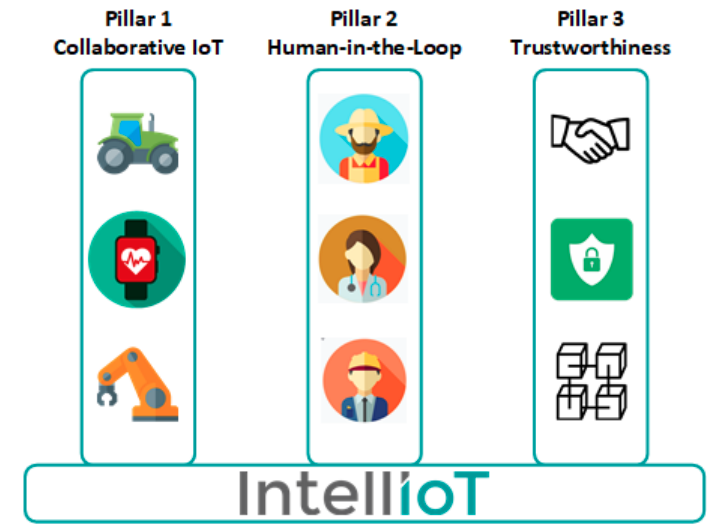
\includegraphics[width=0.8\linewidth]{images/intelliot-pillars.png}
    \caption{The three pillars of \textit{IntellIoT}.}
    \label{fig:intelliot-pillars}
\end{figure}

\subsection{Use Cases}
The above three key component areas are supported by \textit{IntellIoT}'s dynamically managed network and computation infrastructure that, combined, provide resource and edge management, orchestration capabilities, and network choreography, exploiting cutting-edge technologies like 5G.
Moreover, for the pillars to not remain only abstract concepts, various use cases that aim to address real-life problems in three core sectors were developed:

\begin{itemize}
    \item \textbf{Agriculture}: the application of IoT in agriculture could be a life-changer for humanity as we now witness how extreme weather, deteriorating soil, dry lands, and collapsing ecosystems make food production more and more complicated and expensive, not to mention the population growth that increases the demand for resources.
    
    Although ``smart farming'' is already quite popular, \textit{IntellIoT} aims to bring it to the next level thanks to autonomous devices such as self-driving tractors and drones endowed with sensors and actuators.
    However, even though machines perform potentially dangerous, tiring, and repetitive tasks for humans, the latter still play a crucial role in managing the farm.
    Indeed, they can remote control the devices in uncertain situations, refining the Artificial Intelligence models.
    Additionally, human operators are in charge of defining the goals of the farming system, leveraging their experience and knowledge about the domain.
    \item \textbf{Healthcare}: IoT is revolutionizing the healthcare industry, mainly due to remote patient monitoring.
    Indeed, being endowed with specific sensors, devices can track the latter's vital signs and other health metrics and send the collected data to healthcare providers.
    Some examples of such devices are \textit{Continuous Glucose Monitoring} \cite{facchinetti2013real} and \textit{Dissolvable Brain Swelling}\cite{kang2016bioresorbable} sensors or ordinary smartwatches.
    This process improves the patient's quality of life, which does not need to be limited to their home or the hospital and can thus carry on with their regular everyday activities.

    Moreover, continuous monitoring and real-time data sharing allow timely interventions when necessary, and automatic data collection can drastically decrease the time and effort required to retrieve and manage information about the patient.
    Not to mention the opportunities for data analysis and possible Machine Learning models that would support clinicians in being more efficient.
    However, this workflow potentially exposes patients' sensitive information; therefore, we find privacy, security, and trust assurance among the main focuses of \textit{IntellIoT} regarding this use case.
    \item \textbf{Manufacturing}: IoT is one of the core driving forces behind Industry 4.0, which aims to digitalize and automate operational processes counting on as little support as possible from human operators, from the order submission to the delivery of the product.
    Leveraging AI and Machine Learning, robotics, and data analysis, IntellIoT envisions a future with shared manufacturing plants and multiple customers utilizing manufacturing as-a-service.

    According to the latter scenario, an intelligent IoT environment would derive a production plan from data received from a customer.
    Subsequently, the software agents that control the machines would organize according to their role, which is adopted taking into account the machine's capabilities, making it possible to complete the planned steps.
    However, whenever AI is not sufficiently confident about a step, a human-in-the-loop can take over control remotely, providing information that will be learned by the Machine Learning algorithm thanks to continual learning.
\end{itemize}

\section{Domain-Expert Programming}
As already discussed, the crucial role of end-users in the definition of autonomous systems, the importance of their intervention in case of need, and their expertise are utterly unmatched by Artificial Intelligence algorithms and probably will be for a long time.

On top of that, the gap between programmers and end-users regarding domain comprehension is a well-acknowledged issue concerning software development.
Indeed, developers' poor understanding of the domain often results in projects missing their schedules or exceeding their budget, poor-quality software, or even wrong functionalities \cite{5089292}.
To address this critical issue, several techniques have been developed.
For instance, one of the core aspects of Domain Driven Design is \textit{knowledge crunching}, which aims to extract domain knowledge from the experts to reflect it in the code during the subsequent development phases.

On the other hand, a different approach might be taken directly involving domain experts in the programming process.
This kind of user can be defined as professionals in some domain different from computer science who need to use computers in their daily work and often have real needs to perform some programming activities that result in the creation or modification of software artifacts \cite{costabile2003domain}.
Given the latter definition and the premise suggesting the importance of domain expertise, providing domain experts with tools, such as domain-specific languages (DSL) or more user-friendly visual tools, that allow them to ``code'' or configure parts of complex systems feels very natural.
Therefore the need for an intuitive development environment in which users with no proper computer science background can naturally and seamlessly transform their domain knowledge into specifications with low-code (or possibly no-code).

\section{Visual Programming Paradigm}
Multi-Agent Systems is one of the core enabling technologies of the infrastructure of \textit{IntellIoT}.
MAS fit IoT because they tackle the complexity and handle the decentralization of the IoT ecosystem by providing a framework for coordinating the actions of a large number of devices, allowing the latter to communicate and make decisions toward the achievement of a common goal.
Another critical advantage of MAS is their ability to deal with partial knowledge, incomplete and imperfect information, and adapt and reason in real-time, which is crucial in dynamic, uncertain, open, and distributed networks.

However, the high-level expertise required to program agent-based systems hinders the large-scale adoption of MAS.

\subsection{Agent-Oriented Visual Programming}
To facilitate the spread of this technology, efforts have been made to eliminate the entry barrier to MAS development.
One example of such endeavor is the development of an agent-oriented programming paradigm \cite{burattini2022agent}, which enables individuals without coding experience, but with knowledge of specific target domains, to design and (re)configure autonomous software.

This proposal makes the development of software agents easier in two ways:
\begin{itemize}
    \item \textbf{Use of human-oriented abstractions}: the application of the BDI (Belief-Desire-Intention) model, which makes use of concepts such as goals, plans, beliefs, and intentions, allows defining the agent's behavior more naturally, as this paradigm matches more closely people's everyday experience.
    \item \textbf{Use of visual programming techniques}: this project makes use of block-based programming, which is a visual programming paradigm that uses blocks to represent the program's instructions.
    The adoption of a no-code environment allows non-technical users to easily create and modify agents.
\end{itemize}

\begin{figure}[H]
    \centering
    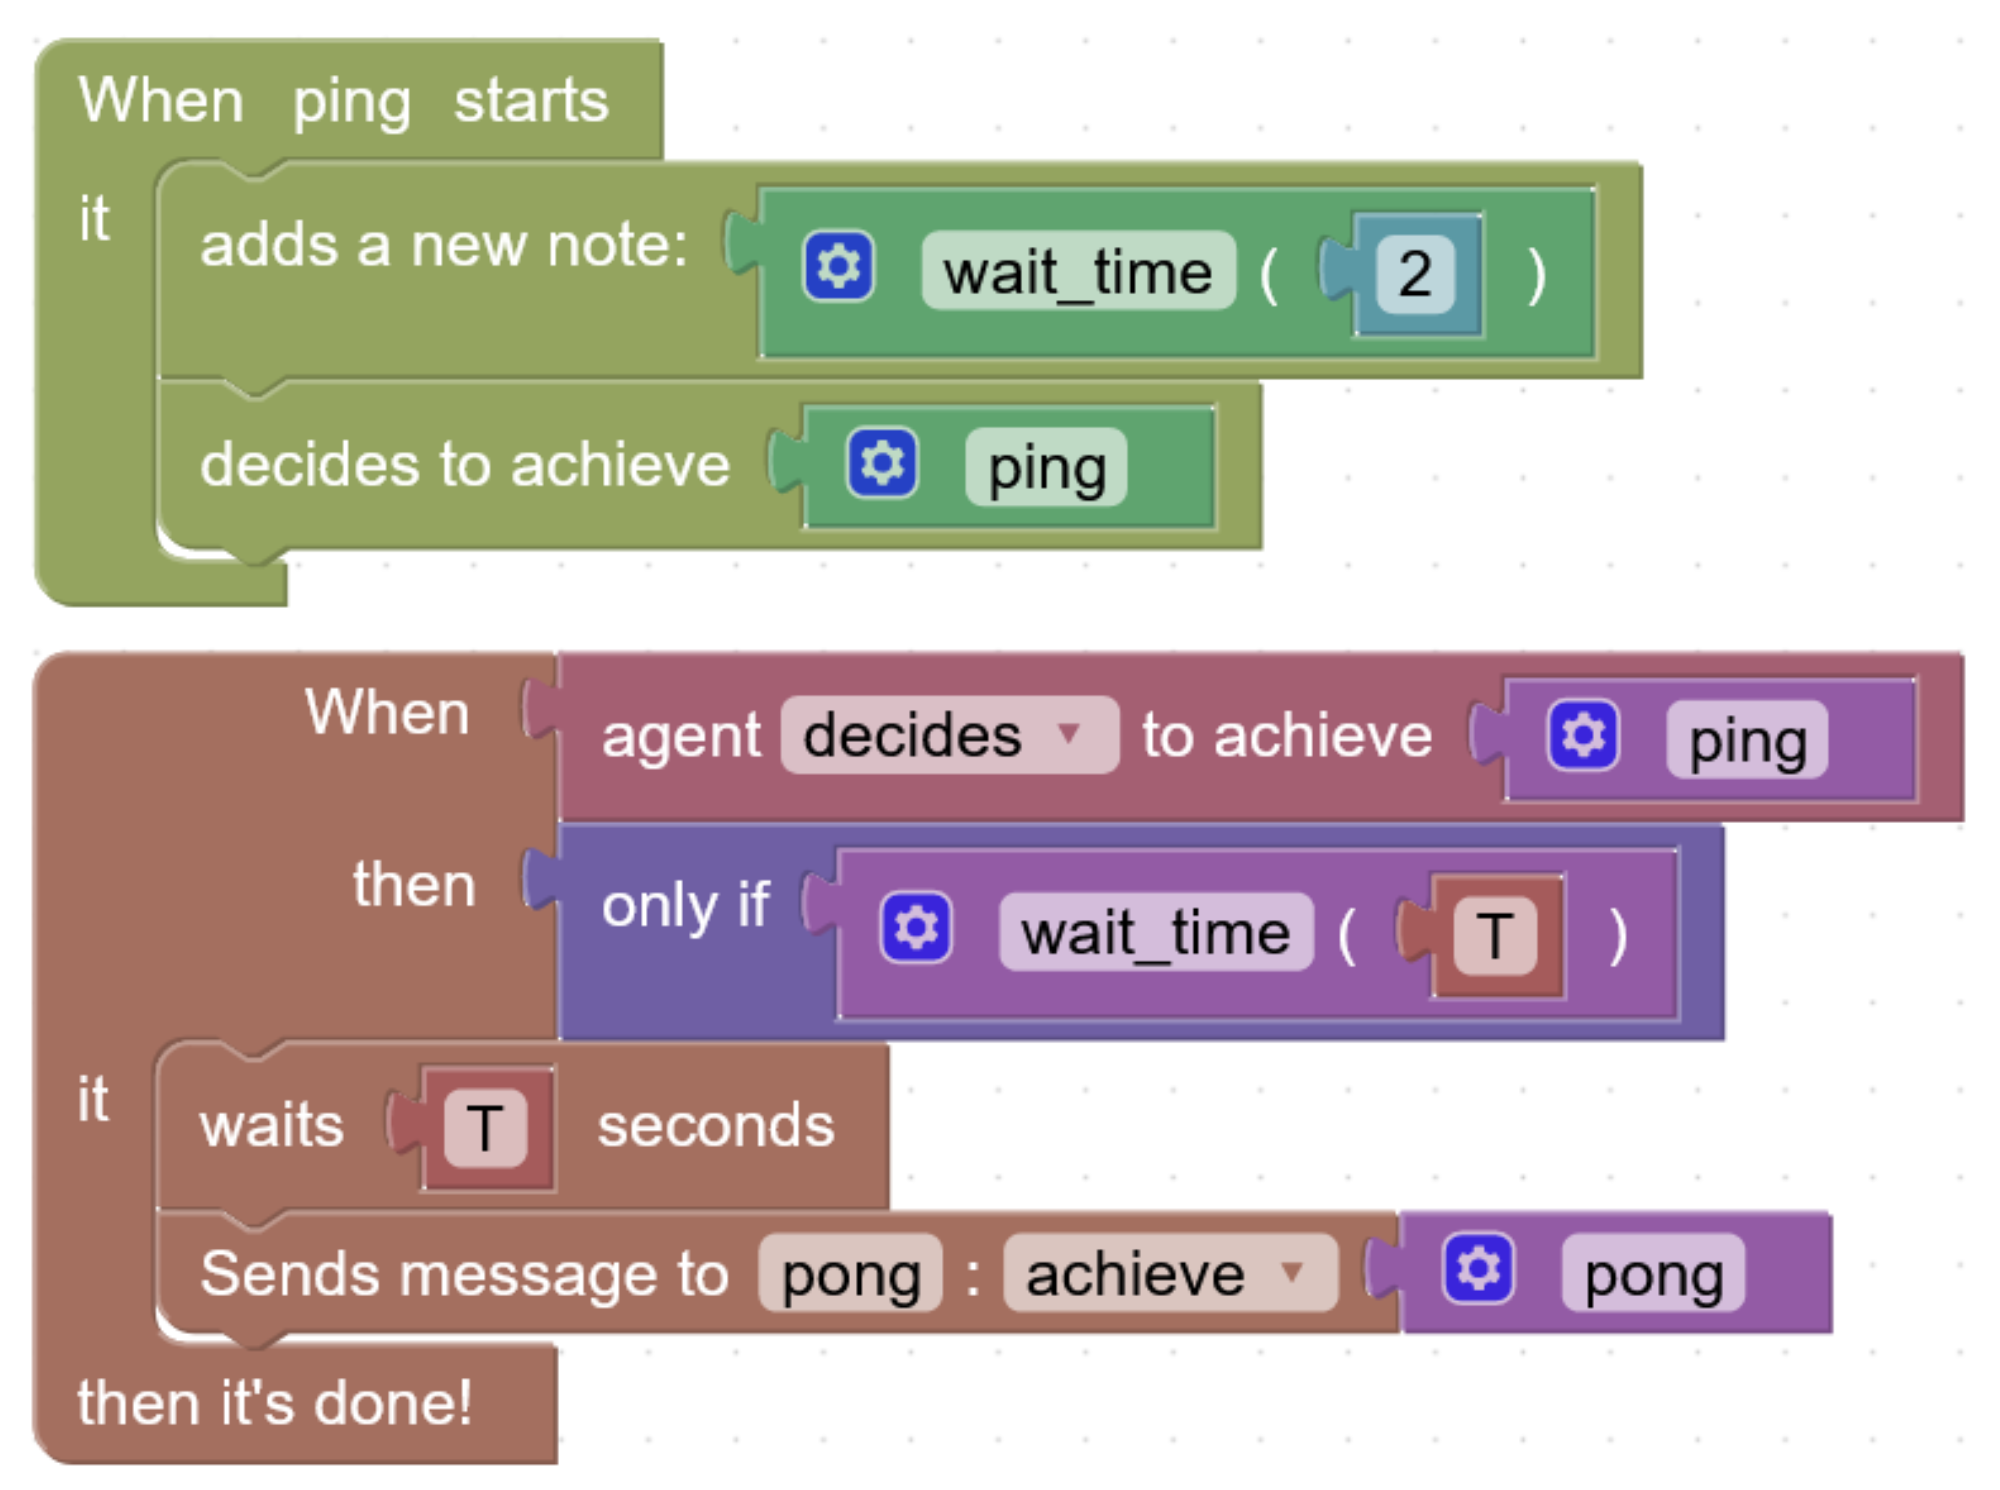
\includegraphics[width=0.9\linewidth]{images/blocks-example.png}
    \caption{Example of a ``ping'' agent implemented with the block language. Adopted from~\cite{burattini2022agent}.}
    \label{fig:blocks-example}
\end{figure}

An example of this work can be found in \cref{fig:blocks-example}, which shows a simple ``ping'' agent.
When started, the agent has a belief that the \texttt{wait\_time} is $2$ seconds, and it has to achieve the goal \texttt{ping}.
In addition, the agent is given instructions on how to achieve the goal through a plan.
The latter states that when the agent decides to achieve the goal \texttt{ping} and knows what the \texttt{wait\_time} is, it should first wait for the time specified in its belief, then send a message to the agent \texttt{pong}.

\subsection{Proposing a Visual Programming Paradigm for Organizations}
Although the above block-based visual development environment is suitable for defining single entities, a level of abstraction to handle the relations among and coordination of the latter is still missing.

When dealing with multiple agents in a MAS, the complexity of the system increases dramatically and the coordination of and interaction among the agents' becomes more and more challenging.
Even though these aspects could be technically represented and managed directly in the mind of the agents, the adoption of adequate abstractions makes the solution dramatically more straightforward and elegant. \cite{boissier2020multi}

Indeed, multiple approaches to organization in MAS have been reported in the literature.
However, all of them require significant coding skills and deep knowledge of the underlying concepts and technologies to be implemented.
Thus, none of these approaches is easy enough to be used by non-technical users such as domain experts.

Therefore, the idea is to design and implement a visual language and a supportive development environment for MAS organizations, which is a novelty to our knowledge.
The core thesis work will be based on studying the existing organization models, with particular attention to the \moiseplus{} model~\cite{10.1145/544741.544858}, and developing an appropriate representation that could provide a suitable tradeoff between the expressiveness of code-based specifications and the ease of use of graphic programming interfaces.

Such a tool would allow domain experts to easily define the organization of a MAS, without the need to write code.
From the \textit{IntellIoT} project's perspective, this would allow addressing more complex scenarios, therefore expanding the range of applications of the IoT framework it aims to create.
Indeed, for the time being, the applications mainly concern the programming of single agents, which reduces the potential of the technology because of the limited interaction and coordination capabilities that this approach allows.

Moreover, the adoption of a visual language would provide a valuable tool to monitor and debug the system, learn the concepts behind the technology, and hopefully bring new users to the field of MAS.

The thesis project will end with the implementation of a prototype that allows users to define the organization of a MAS by using the developed visual language.
In particular, the aspects of the organization that will be covered, and thus the users will be able to specify, are:
\begin{itemize}
    \item \textbf{Structure}: This part is responsible to define how agents should be organized in the system, i.e., how they should be grouped and how they should interact with each other;
    \item \textbf{Behavior}: This aspect regards the definition of the common goals that the agents have to achieve, and how agents should coordinate their actions to achieve them;
    \item \textbf{Rules}: This concept concerns the norms that regulate the agents' behavior.
    In particular, they represent what agents are and are not allowed to do, or what they are obliged to do.
\end{itemize}

To evaluate the developed tool, a qualitative evaluation is planned to receive feedback for the developed language and development environment and to study how non-technical users solve problems by exploiting the visual language.
Moreover, the visual language will be used and tested with a real-world scenario to evaluate the correctness of the resulting MAS.
This twofold evaluation will allow assessing the user-friendliness of the developed tool on the one hand, and its expressivity and potential on the other.

Before proceeding with the technical description of the designed language and the implemented prototype, the following chapter provides an introduction to the background of the main technologies and research topics explored in the thesis project.
\chapter{Background}

\section{Multi-Agent Oriented Programming}
The concept of a software agent can be traced back to the early days of research into Distributed AI in the 1970s when Carl Hewitt proposed the concurrent Actor model.
In his paper, he introduced the concept of a self-contained, interactive, and concurrently-executing object which he termed ``actor''.
The latter is a computational agent with a mail address and behavior. Actors can communicate by message-passing and carry out their actions concurrently. \cite{hewitt1977viewing}

\subsection{What is an Agent?}
The term ``agent'' quickly spread to heterogeneous research fields; therefore, there is no commonly agreed definition for it.
However, a generally accepted description of what an agent is is the following by Wooldridge \cite{490039}:
\begin{quote}
    \textit{An agent is a self-contained program capable of controlling its own decision-making and acting, based on its perception of its environment, in pursuit of one or more objectives.}
\end{quote}
To sum up, we can identify a set of features that an agent should possess:
\begin{itemize}
    \item \textbf{Autonomy}: agents should be able to perform most of their tasks without the direct intervention of humans or other agents, and they should encapsulate control over their actions and internal state
    \item \textbf{Social ability}: agents should be able to interact with each other and possibly humans to complete their tasks.
    \item \textbf{Responsiveness} (situatedness): agents should perceive their environment and respond to changes in it.
    \item \textbf{Proactiveness}: agents should exhibit opportunistic, goal-directed behavior and take the initiative when appropriate.
\end{itemize}

During the first years, the research concentrated on interaction and communication among agents, decomposition and distribution of tasks, and coordination and cooperation.
The goal was to specify, analyze, design, and integrate systems containing multiple collaborative agents.

\subsection{Multi-Agent Systems}
Multi-Agent Systems have been studied as a per se field since the 1980s and gained widespread recognition in the 1990s.
Since then, international interest in the topic has grown enormously as agents are considered an appropriate paradigm to exploit the possibilities presented by massive open distributed systems.
Moreover, MAS seem to be a natural metaphor for understanding and building a wide range of what we might call \textit{artificial social systems}. \cite{wooldridge2009introduction}

According to the \textit{Alan Turing Institute} \cite{turing}
\begin{quote}
    \textit{A Multi-Agent System consists of multiple decision-making agents which interact in a shared environment to achieve common or conflicting goals.}
\end{quote}

\begin{figure}[H]
    \centering
    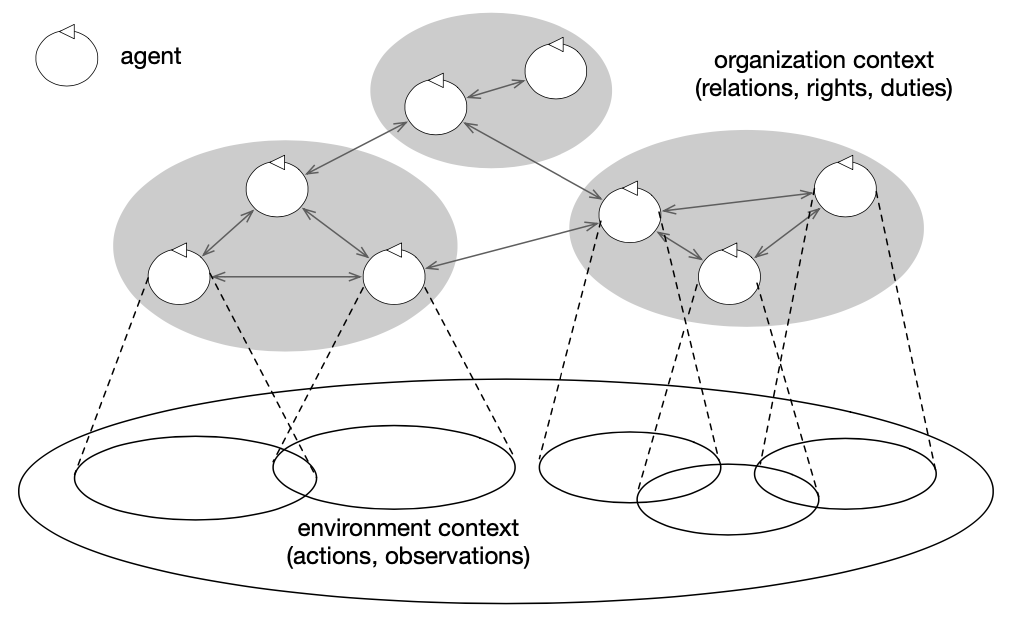
\includegraphics[width=0.9\linewidth]{images/multi-agent-systems.png}
    \caption{A representation of Multi-Agent Systems. \cite{jennings2000agent}}
    \label{fig:multi-agent-systems}
\end{figure}
As it can be noticed in \cref{fig:multi-agent-systems}, MAS are composed of the environment and agents existing within it that are bonded by relations.

\subsubsection{Environment}
The environment in MAS presents two facets:
\begin{itemize}
    \item \textit{The environment as the ``external world''}.
    Agents become aware of the context they are immersed in and its dynamics by perceiving the environment through sensors.
    Moreover, they pursue their goals through actions performed by actuators that aim at modifying the environment, eventually reaching the latter's desired state.
    \item \textit{The environment as a medium for coordination}
\end{itemize}

\section{Hypermedia Multi-Agent Systems}
\section{Organizations in Multi-Agent Systems}

\chapter{Requirements}
\section{Functional Requirements}
\section{Non-Functional Requirements}
\chapter{Design}

\section{A Visual Language for Organizations}
\subsection{Organization Structure}
\subsection{Collective Goals}
\subsection{Goals Allocation}

\section{Main Components}
\subsection{Web-Based IDE}
\subsection{Storage Backend}

\chapter{Development}\label{development}

In the following chapter, the development process that followed the design phase and brought to the creation of the prototype of the whole system is described.

Some technological constraints were imposed from the requirements and the design phase.
In particular, the need for a lightweight Web application that didn't have to be installed on the user's machine and, from the MAS infrastructure point of view, the need to adhere to the JaCaMo platform, therefore to produce XML \moise{} specifications.

The development process was divided into three main parts.
First, the Web IDE was implemented to get continuous and fast feedback about the visual language.
Second, the backend and the specifications storage were developed to provide persistence to the organizations created by users.
Finally, the Web IDE was integrated with the runtime environment to allow the user to access information about the running agents and deploy the organizations.

The important details and choices about the implementation of the main component of the systems are described in the following sections.

\section{Web-based IDE}
Given that the main goal of the project is to provide non-technical users with an easy and intuitive tool to create and run organizations, the Web IDE is probably the most important component of the system together with the visual language.
Therefore, when users are confronted with the UI of the IDE they should be able to clearly understand what each component of the interface means and how to use it without any detailed explanation.

\begin{figure}
    \centering
    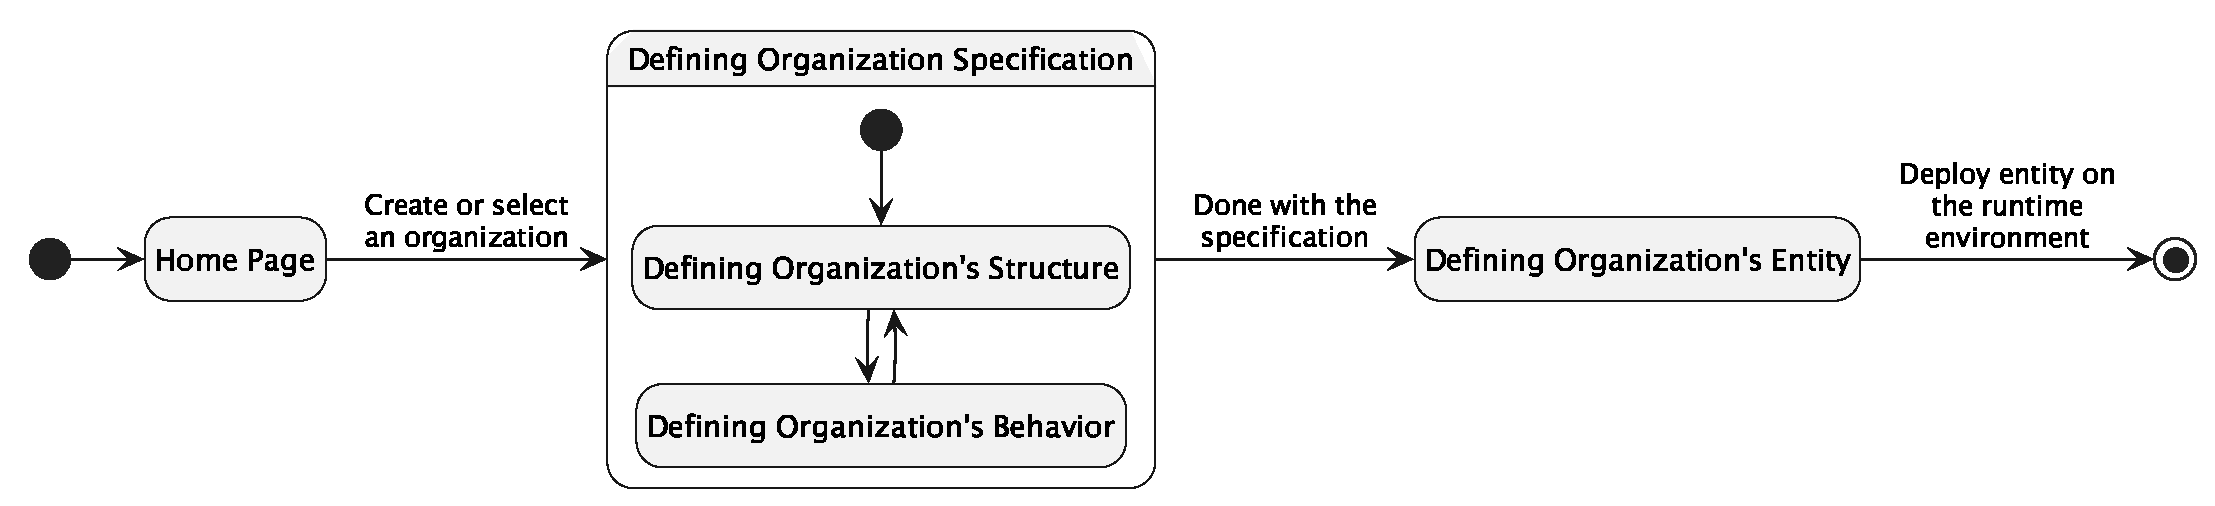
\includegraphics[width=\linewidth]{images/web-ide.eps}
    \caption{Typical workflow of a user utilizing the Web-based IDE.}
    \label{fig:ide}
\end{figure}

\subsection{Web User Interface}
As a starting point for the design of the UI, the typical workflow of a user that wants to create an organization is considered.

As shown in \cref{fig:ide}, the user starts by either creating a new organization or selecting an existing one.

Then, the user can define or edit the organization specification by using the designed visual language.
In particular, the user specifies the structure and the expected behavior of the organization in an iterative way.
Indeed, it is important to avoid sequentiality in the process as the user should feel free to easily navigate through the two separate diagrams and continuously modify them as the organization evolves.

Once the specification is ready, the user can define the organization entity by assigning the roles to the running agents. Finally, the organization can be deployed on the runtime environment and enforced on the agents.

Therefore, the final UI of the Web IDE consists of four main pages:
\begin{itemize}
    \item \textbf{Home Page} where the user can specify the name of the organization and create it or select an existing one.
    \item \textbf{Structural Diagram} where the user can define the structure of the organization.
    \item \textbf{Functional Diagram} where the user can define the expected behavior of the organization.
    \item \textbf{Entity Definition} where the user can assign the roles to the running agents and deploy the organization.
\end{itemize}

In \cref{fig:ide-structural-all} the UI of the Structural Diagram is shown.
As can be seen, the left panel contains the available elements that can be used to create the organization structure.
Indeed, the user can create new roles choosing whether they are concrete or abstract, and new groups.
Once a component has been created, it can be moved around the diagram and modified by clicking on it.
The click on a component opens a side menu that allows the user to edit the properties of the selected component.
In particular, \cref{fig:ide-structural-side} shows the side menu for the role \texttt{r1}.
Here the user can specify which role, if any, the selected role extends from, which group it belongs to, and the cardinality of the role in the group, i.e. the minimum and maximum number of agents that can be assigned to the role.

\begin{figure}
    \centering
    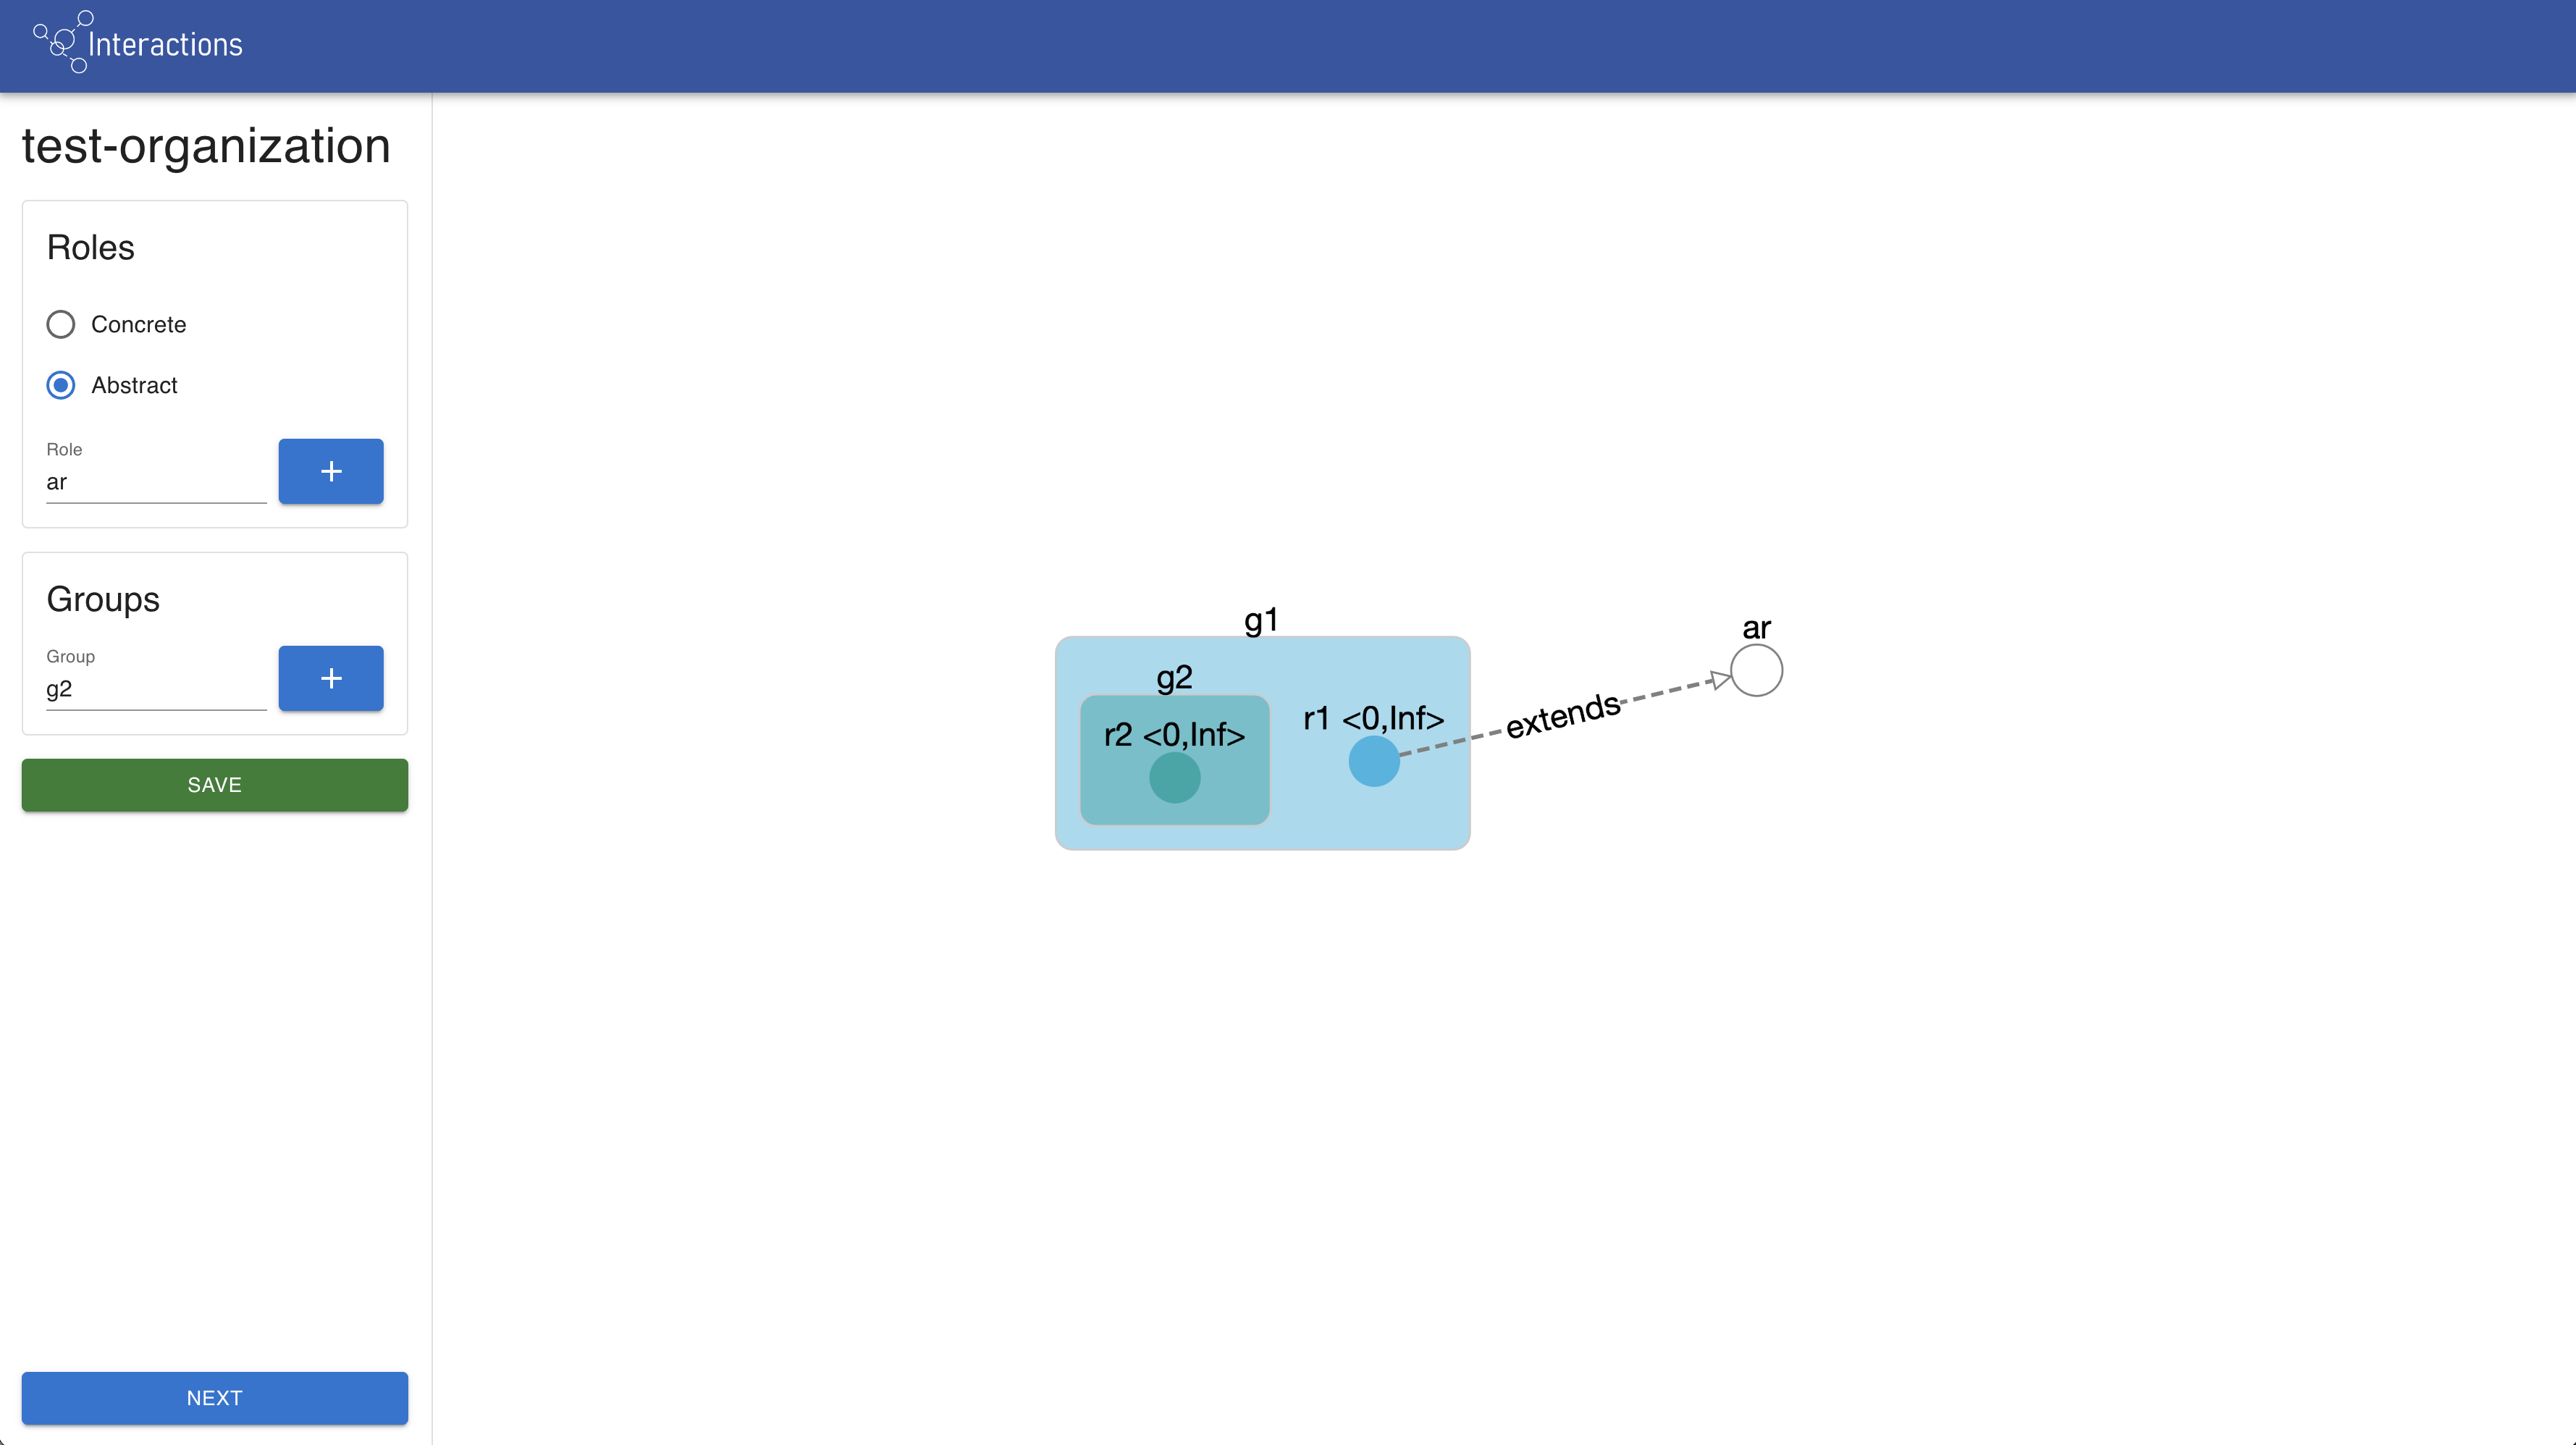
\includegraphics[width=\linewidth]{images/ide/structural.png}
    \caption{Structural Diagram of the Web IDE.}
    \label{fig:ide-structural-all}
\end{figure}

\begin{figure}
    \centering
    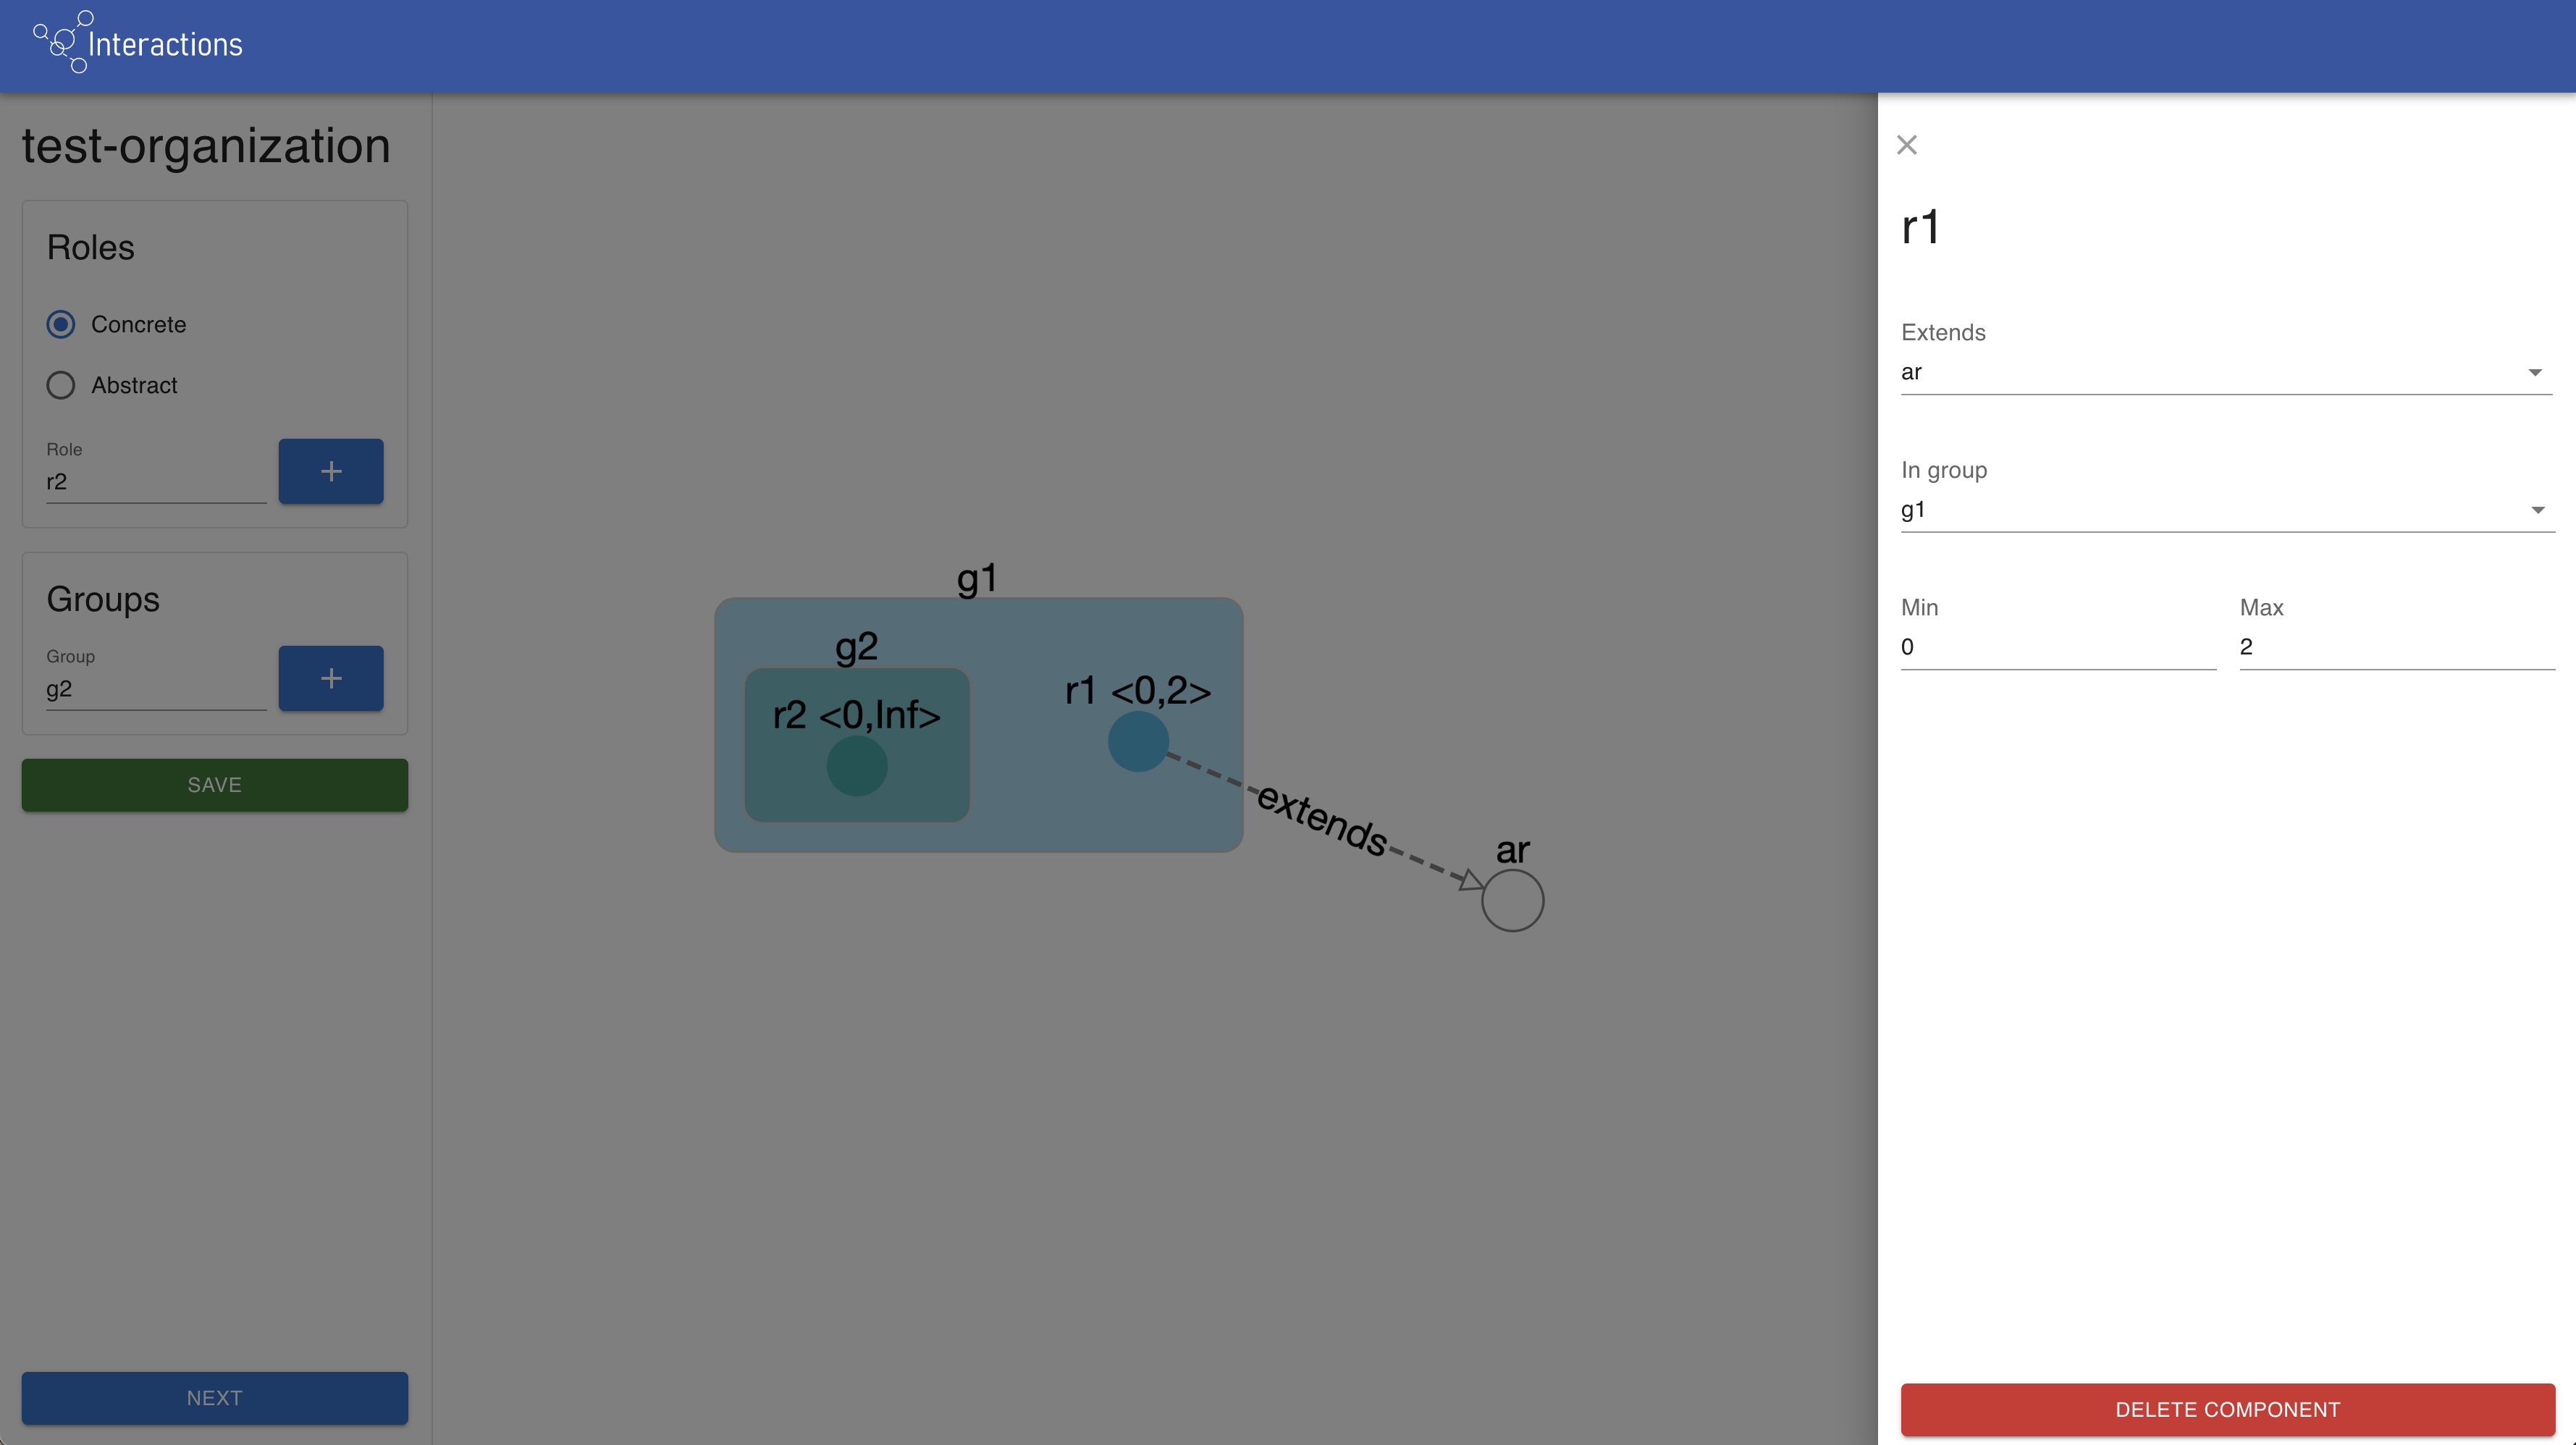
\includegraphics[width=\linewidth]{images/ide/structural-side.png}
    \caption{Detail showing the side menu in the Structural Diagram of the Web IDE.}
    \label{fig:ide-structural-side}
\end{figure}

\subsection{Technologies}
The following section describes the main technologies used to implement the Web IDE.

Since the component is based on Web technologies, the main two languages available for the implementation of the client-side logic are \textit{JavaScript}~\footnote{\url{https://developer.mozilla.org/en-US/docs/Web/javascript}} and \textit{TypeScript}~\footnote{\url{https://www.typescriptlang.org/}}.
The latter was created to address problems coming with developing large-scale applications, introducing static typing and object-oriented features.
Typescript's type-checking makes it easier to find and fix bugs, therefore, it was chosen as the language for the implementation of the Web IDE.

Moreover, a client-side framework was used to implement the Web-based IDE.
The main reason for this choice is that frameworks provide a set of tools that simplify the development of interactive Web applications.
They allow the developer to create reusable components that encapsulate the logic and the UI of a specific part of the application, therefore helping to divide the latter into smaller and more manageable parts and keeping the code clean and organized.
The one chosen for this project is \textit{React}~\footnote{\url{https://reactjs.org/}}.
Although there is no strong motivation for why it was preferred over others, React is probably the most popular, therefore, possible new contributors to the project will be more likely to be familiar with it.

To further facilitate the development of the UI, the \textit{Material-UI}~\footnote{\url{https://mui.com/}} library was used.
It implements Google's \textit{Material Design} and it provides a set of tested prebuilt components that are ready to be used in the application.

Finally, to make the implementation of the diagrams easier, the \textit{Cytoscape}~\footnote{\url{https://js.cytoscape.org/}} library was used.
It is a modular graph library that provides a set of tools to create and manipulate graphs and diagrams.
Using the library, together with a few extensions, made it possible to provide a simple and intuitive way to create and edit the diagrams.

\subsection{Code Generation}\label{sec:code-generation}
Since the specifications created by the user with the Web IDE have to be compatible with the JaCaMo platform, and in particular, with \moise{}, the diagrams have to be translated into XML files.
Equally important, actual \moise{} XML specification files have to be correctly parsed and translated into the corresponding visual representations.

Once the design phase of the different components of the visual language was in an advanced stage, the actual implementation of the code generation started.

The decision was to first implement the components that are present in both the Structural and Functional Diagrams.
This allowed for having a core domain that is unlikely to change in the future and that could be used as a starting point for both the translation into the visual components and XML tags.
In particular, the core domain consists of the components shown in \cref{fig:uml-core-domain}.

\begin{figure}
    \begin{subfigure}[h]{0.6\linewidth}
        \centering
        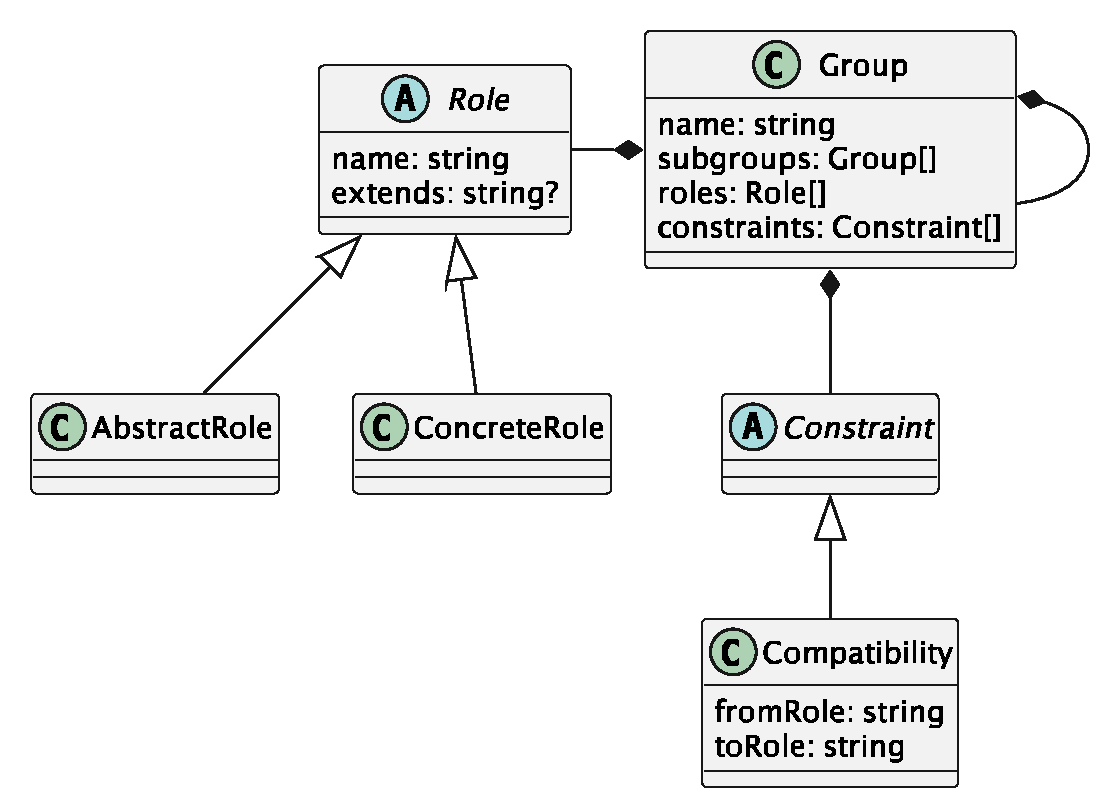
\includegraphics[width=0.9\linewidth]{images/uml/structural-uml.eps}
        \caption{Structural Diagram Core Domain.}
        \label{fig:uml-structural}
    \end{subfigure}
    \begin{subfigure}[h]{0.3\linewidth}
        \centering
        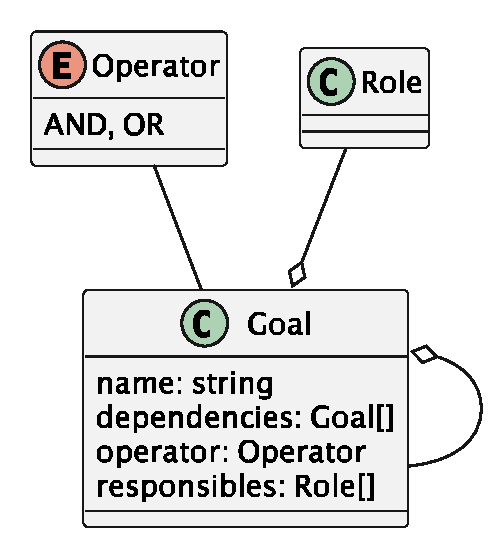
\includegraphics[width=0.9\linewidth]{images/uml/functional-uml.eps}
        \caption{Functional Diagram Core Domain.}
        \label{fig:uml-functional}
    \end{subfigure}
    \caption{UML class diagrams of the core domain.}
    \label{fig:uml-core-domain}
\end{figure}

Specifically, the system keeps track of the components of the diagrams and the relations between them in a list.
The latter is then taken as input by a \texttt{serialize} function that transforms the list into an XML string.
On the other hand, an analogous process is performed when loading an XML specification.
The \texttt{deserialize} function takes the XML string as input and transforms it into a list of components.
In \cref{lst:code-serialization} and \cref{lst:code-deserialization} are shown the functions for the code generation and parsing of the roles inside a group, respectively.

\begin{figure}[H]
    \lstinputlisting[language=Typescript,label={lst:code-serialization},caption={Code generation for the roles inside a group.}]{code/serialization.ts}
\end{figure}

\begin{figure}[H]
    \lstinputlisting[language=Typescript,label={lst:code-deserialization},caption={Parsing of the XML specification of a role inside a group}]{code/deserialization.ts}
\end{figure}

As far as the goal dependencies are concerned, a one-to-one mapping was not possible since the visual language's semantics differs from the one used by \moise{}.
Specifically, the visual language does not allow for the creation of plans and subgoals that are not associated with a specific goal with a plan operator.
In order to overcome this incompatibility, the \textit{depends-on} concept of \moise{} was used.
Although it is usually not directly used in the XML specifications, \textit{depends-on} is a fundamental concept of \moise{} which plans and subgoals are built upon.

Therefore, this concept is used as a mapping between the visual language and the XML syntax.
In particular, when expressing the \textit{and} dependency, a simple \textit{depends-on} tag is created between the two goals.
On the other hand, when expressing the \textit{or} dependency, an intermediate goal is created with a \textit{choice} plan.

For instance, in \cref{lst:goals-and} is shown the XML translation of an \textit{and} dependency between the goals \textit{g1}, \textit{g2} and \textit{g3} of the type:
$$g3 = g1 \wedge g2$$
whereas in \cref{lst:goals-or} is shown the XML translation of an \textit{or} dependency between the goals \textit{g1}, \textit{g2} and \textit{g3} of the type:
$$g3 = g1 \vee g2$$

\begin{figure}
    \lstinputlisting[language=XML,label={lst:goals-and},caption={XML translation of an \textit{and} dependency.}]{code/goals-and.xml}
\end{figure}

\begin{figure}
    \lstinputlisting[language=XML,label={lst:goals-or},caption={XML translation of an \textit{or} dependency.}]{code/goals-or.xml}
\end{figure}

\section{Storage \& Backend}
Organizations can be saved persistently to be later recovered and edited.
This feature is fundamental for the Web IDE since writing a specification is commonly an iterative process that may require the domain expert to edit some parts of an organization either for bug-fixing or to add new features.

\subsection{Storage}

Since the visual programming environment is based on Web technologies, centralized server-side storage was the most natural choice.
Looking at the system architecture in \cref{fig:architecture}, the \textbf{Specifications' Storage} component is responsible for this functionality.

The storage uses a \textit{MongoDB}~\footnote{\url{https://mongodb.com/}} database to store the generated XML specifications.
For the time being, the database does not store the information about the diagrams, such as the position of the components that would make it easier to load the organization in the same state as it was saved.

Moreover, there is no separation between the specifications created by different users, therefore, in a production environment some form of authentication would be necessary.

Finally, a further improvement of the storage component would be to also allow the user to save organization entities, keeping track of which specific configurations of the organization in different scenarios.

\subsection{Backend}
Since, as already mentioned, the Web IDE is based on Web technologies, a backend seemed the most natural choice to make the frontend and the storage communicate.

The backend was implemented using the \textit{Kotlin}~\footnote{\url{https://kotlinlang.org/}} programming language and the \textit{VertX}~\footnote{\url{https://vertx.io/}} library.
The latter is a reactive library that allows the developer to write asynchronous code and build Web servers quickly.
It was chosen because the research group in St.\ Gallen already had some experience with it, therefore, it would be easier to maintain for other developers.
In particular, the projects built by the team use \textit{Java}~\footnote{\url{https://java.com/}} as the programming language, therefore, the choice of \textit{Kotlin} was a fair tradeoff that allowed using a language that is similar to \textit{Java} but with a more modern and concise syntax.

The backend exposes an HTTP API that allows the frontend to communicate with the storage.
The API that is currently implemented is here described:
\begin{itemize}
    \item \texttt{GET /organizations/:name}: returns the XML specification of the organization with the given name.
    \item \texttt{POST /organizations/:name}: saves the XML specification present in the body to the storage.
    \item \texttt{PUT /organizations/:name}: updates the organization with the given name, substituting it with the XML specification present in the body.
\end{itemize}
Since the \texttt{GET} route returns the XML specification, the runtime environment can also use it as a way to retrieve the specification in a resource-oriented fashion.

\section{Running Organization Entities}
In order for users to be able to run the organizations they create, the Web IDE has to be able to communicate with the runtime environment.
Specifically, it needs information about the running agents to assign them to the correct roles and, subsequently, it needs to enforce the organization on said agents.

\subsection{Runtime Environment}
As already mentioned, the runtime environment, which is based on the JaCaMo platform, contains all the running agents and the deployed artifacts.

This component is currently being developed by the research group in St.\ Gallen.
The name of the platform is \textit{Yggdrasil}~\footnote{\url{https://github.com/Interactions-HSG/yggdrasil}}, which comes from the mythological tree of life, and it aims at providing uniform interaction among heterogeneous agents thanks to Hypermedia MAS.
The idea is to model an environment based on the Agents \& Artifacts metamodel through hypermedia and Web technologies, achieving scalability and uniform access to resources.

Yggdrasil exposes a REST-like API that allows users and agents to navigate the environment and the existing workspaces where artifacts and their operations are described with the Thing Description standard since the model perfectly fits the Agents \& Artifacts metamodel.
Moreover, the platform's API also allows the user to run agents and create and deploy artifacts.

The format used by Yggdrasil to describe the resources in the environment is the \textit{Turtle}~\footnote{\url{https://w3.org/TR/turtle/}} format.
The latter is a textual syntax for RDF that allows a knowledge graph to be represented in a compact and natural text form.

\subsection{Running Agents}
Agents in Yggdrasil, just like artifacts, are contained in workspaces.
Therefore, to get the list of agents that are currently running, the Web IDE has to operate on a workspace and retrieve the list of resources that are contained in it.

By performing a \texttt{GET} request to the \texttt{/workspaces} endpoint, specifying the workspace name in the URL, the Web IDE can retrieve a Turtle representation of the workspace; a short example of the response is shown in \cref{lst:turtle-workspace}.
As can be seen, the workspace, which is the subject of all the triples, \textit{directlyContains} \texttt{hypermedia\_body\_1} and \texttt{hypermedia\_body\_2} which represent two agents currently running.

\begin{figure}
    \lstinputlisting[language=Turtle,label={lst:turtle-workspace},caption={Detail of the Turtle representation of a workspace.}]{code/turtle-workspace.ttl}
\end{figure}

Therefore, the Web IDE can parse the Turtle representation and extract the list of agents that are currently running, filtering them from all the other resources that are contained in the workspace.
Since this list is composed of URIs, \texttt{GET} requests to them can be performed to retrieve the Turtle representation of the agents.
The response of the \texttt{GET} request to the agents provide useful information for the user such as the name of the agents that can be used to recognize them and assign them to the correct roles.

\subsection{Artifacts Creation}
Artifacts in Yggdrasil can be created by performing a \texttt{POST} request to the \texttt{workspace/:workspaceName/artifacts} endpoint, specifying all the necessary information in the body of the request.
For instance, the body should contain the type of artifact that is being created, the name of the artifact, and possible initial parameters that the artifact may need.

As far as the organizational artifacts are concerned, the types of artifacts available are the same as the ones described in \textsf{ORA4MAS}, therefore \texttt{OrgBoard}, \texttt{GroupBoard}, \texttt{SchemeBoard}, and \texttt{NormativeBoard}.
Once the \texttt{OrgBoard} artifact is created, the most correct way to generate the other artifacts is through an action exposed by it.
In particular, the \texttt{OrgBoard} artifact exposes the \texttt{createGroup} and \texttt{createScheme} actions that can be used to create the other artifacts.
A \texttt{NormativeBoard}, on the other hand, is automatically generated when a \texttt{SchemeBoard} is linked to a \texttt{GroupBoard}.

Therefore, to correctly instantiate the organizational artifacts and have them refer to the same organization, the Web IDE has to perform a \texttt{POST} request to the \texttt{workspace/:workspaceName/artifacts} endpoint to create the \texttt{OrgBoard} artifact, and then, once the latter is created, perform a \texttt{POST} request to the \texttt{workspace/:workspaceName/artifacts/:orgName/create*} endpoint to create the other artifacts.

\subsection{Organizations' Deployment}
Deploying an organization is a process that includes the creation of the correct organizational artifacts and the adhesion of the agents to the organization, i.e. playing the established roles in the prescribed groups.

\begin{figure}
    \centering
    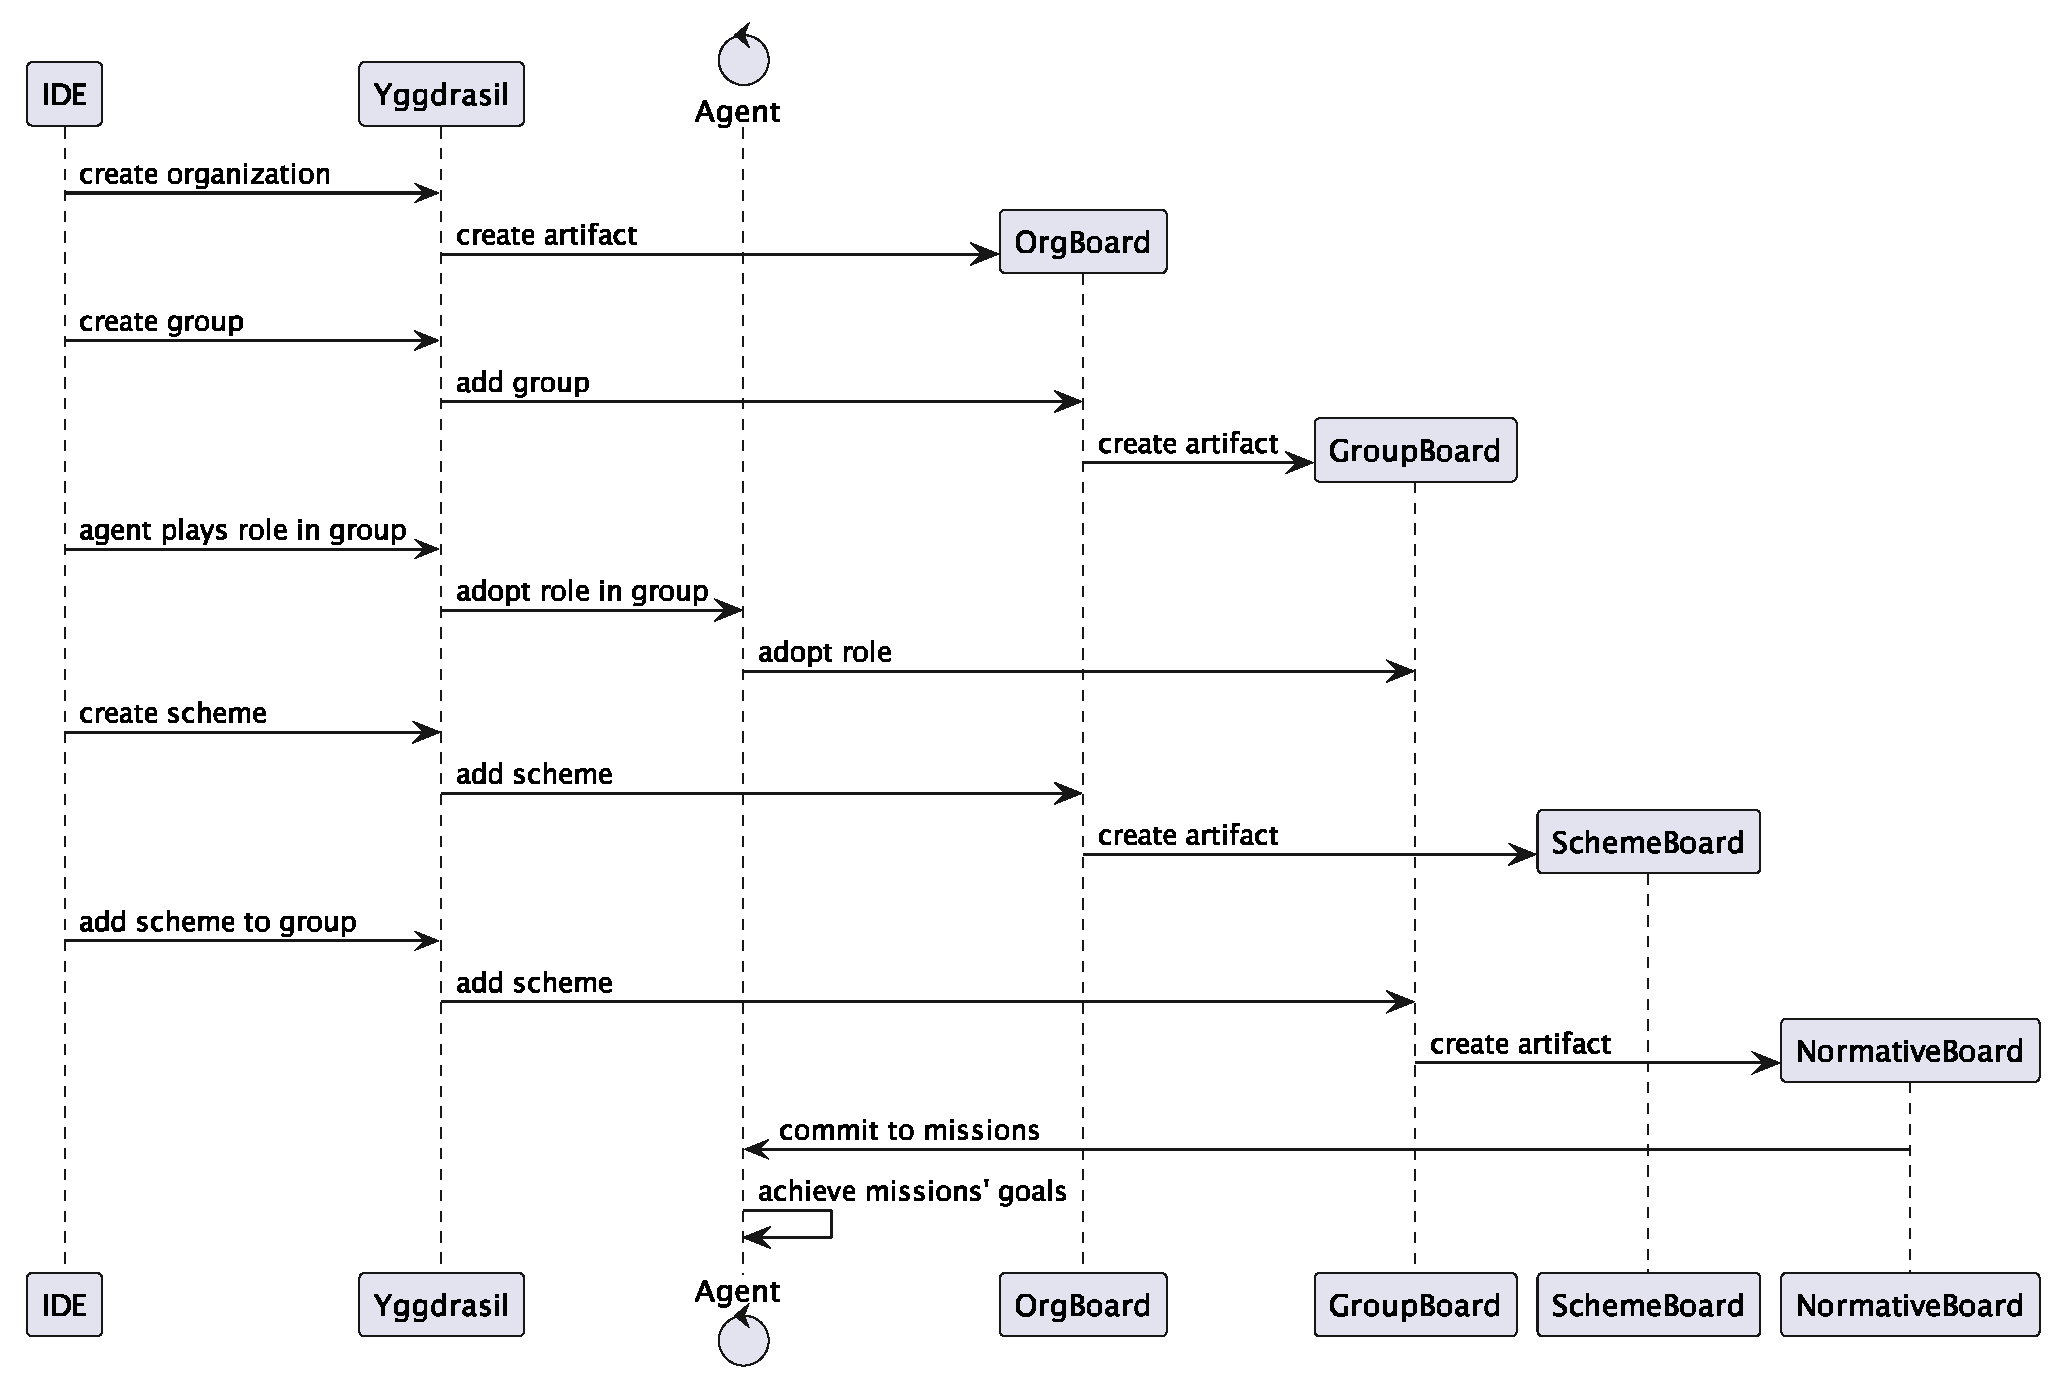
\includegraphics[width=\textwidth]{images/uml/org-creation.eps}
    \caption{Sequence UML diagram of the deployment of an organization. The responses are omitted to improve the readability.}
    \label{fig:org-creation}
\end{figure}

In \cref{fig:org-creation} the typical deployment process of a simple organization is shown.
\begin{enumerate}
    \item The Web IDE first sends a request to Yggdrasil to create the \texttt{OrgBoard} artifact, which is the artifact that represents the organization.
    \item Once the artifact is ready, the Web IDE creates the groups specified in the organization entity.
    For each group, a \texttt{createGroup} request is sent to the \texttt{OrgBoard} artifact, which creates the \texttt{GroupBoard} artifact that represents the group.
    \item The next step involves telling the agents to play the roles specified in the organization entity inside the groups.
    To do so, the Web IDE sends a message to the agents, which know how to send a request to the \texttt{GroupBoard} artifact to play the role.
    \item Subsequently, the Web IDE sends a request to create the scheme of the organization.
    This request is sent to the \texttt{OrgBoard} artifact, which creates the \texttt{SchemeBoard} artifact that represents the scheme.
    \item Finally, the Web IDE sends a request to add the scheme to the groups.
    This request creates a link between the \texttt{SchemeBoard} artifact and the \texttt{GroupBoard} artifacts and a \texttt{NormativeBoard} is automatically generated.
    \item Since the agents are listening to events generated by the \texttt{GroupBoard} artifacts, they will receive a notification telling them to achieve the goals specified in the scheme.
    \item If the agents are obliged to achieve the goals, they will proceed to do so.
    On the other hand, if the agents are permitted to achieve the goals they will do so only if they have an interest in it.
\end{enumerate}

% \section{DevOps}
% In order to 

% In order to make the deployment of the whole system easier, every component has been containerized using \textit{Docker}~\footnote{\url{https://www.docker.com/}}.
% Therefore, a \texttt{Dockerfile} was created for each component, except for the storage component, which only needed the \texttt{mongo} image.

% Moreover, since running every single container with its parameters would be tedious and error-prone, a \textit{Docker Compose}~\footnote{\url{https://docs.docker.com/compose/}} file was created to make the deployment possible with a single command.

% Indeed, the \texttt{docker-compose.yml} file contains all the necessary information to run the whole system,
% such as the images and the build files to use, the ports to expose, the environment variables to set, and the volumes to mount.
% What is more, it takes care of creating a bridge network that allows the containers to communicate with each other.

\chapter{Evaluation}\label{chap:evaluation}
After developing a working prototype of the whole system, the next step was to prove that the solution satisfies the requirements.

This chapter describes the evaluation of the developed system.
In particular, the evaluation is divided into two parts:
\begin{enumerate}
    \item the first part involves the use of the developed system to solve a real-world problem;
    \item the second part is a qualitative evaluation of the developed visual language and development environment by users;
\end{enumerate}
As already mentioned, this twofold evaluation approach allows for assessing the user-friendliness of the development environment and the effectiveness of the visual language on one hand, and the expressivity and correctness of the latter on the other.

\section{Case Study}
In order for users to have a real-world problem to solve, both during the design phase with the focus group and during the evaluation phase with the end users, a use-case scenario was developed.

\subsection{Smart-Farming Scenario}

Since the \textit{IntellIoT} project already defines three sectors of application, namely \textit{Agriculture}, \textit{Healthcare} and \textit{Manufacturing}, the most natural choice was to use one of them to frame the case study.
The \textit{Agriculture} sector was chosen because it involves concepts that are easy to understand even for non-experts and it is possibly the most diverse.

Therefore, the case study was developed around the \textit{Smart Farming} scenario where the aim is to define an organization for a typical farm that adopts IoT technologies. Here is reported the text of the scenario:

\begin{quote}
Thanks to his investments, the farmer obtained the most cutting-edge technology machines to make his life easier.
After obtaining this technology, the farmer wants to organize the management of the daily chores of his ``smart farm'' by exploiting the machinery he possesses, which includes a self-driving tractor, multiple drones, an automatic irrigation system, and devices to take care of the animals.

With the acquired machinery, the farmer must irrigate the fields, which is highly demanding.
Therefore, the farmer purchased drones to improve the process of checking the soil and gathering information such as temperature and humidity, which the irrigator can use to calculate the amount of water needed.
The drones not employed for the former tasks will eliminate the moths and bugs that haunt the cultivation.

In addition, the farm always has a field that is currently not used to grow any crop.
However, the tractor must still plow the soil in that field.
To perform this function, it will need a set of waypoints.
The tractor can either have them computed by a drone flying over the field or as direct input from the farmer.

Finally, the farmer wants to harvest mature fruit and vegetables (we can assume that the tractor knows how to harvest).
After the harvest, the tractor can spray the field with pesticides to protect the crop.

As far as the animals are concerned, the farmer wants to feed them and have a daily health check-up for every animal. 
Moreover, he wants to collect the eggs from the hens and milk the cows and the goats.
It is worth mentioning that, during years of experience, the farmer noticed that feeding the animals before their health check-up makes them quieter, and the cows and the goats calmer when they get milked.
\end{quote}

\subsection{Use-Case Analysis}
Although not only one solution is possible for this example, here a reference one is described.
The approach to the problem, analogous to the one explicitly suggested to the focus group and to end users, consists of the following steps:
\begin{itemize}
    \item identify the roles of the organization;
    \item identify the groups of the organization;
    \item identify the tasks to be performed and possible relations between them;
    \item identify which roles are responsible for the tasks.
\end{itemize}
In particular, the approach used to solve the case study follows some simple guidelines.
As far as task decomposition is concerned, there could be different reasons why a task may be split into subtasks.
For instance, a task may be too complex to be performed by a single agent since it needs the capabilities of multiple agents.
Another reason may be that a task takes too much time to be performed atomically and it is better to split it into smaller tasks.
Moreover, a task may be decomposed into subtasks to use the achievement of a subtask as a precondition for the achievement of another task.
Finally, a task may be split into subtasks to allow for parallel execution of the subtasks by multiple agents.

On the other hand, when it comes to the definition of the roles, the approach mainly relies on the identification of a set of capabilities that the agent playing that role should provide in order to perform the tasks assigned to it.
For instance, referring to the ``write paper'' example in \cref{fig:moise-visual}, the role of the \texttt{writer} is defined by the capability of writing the sections of a paper, therefore agents playing that role can successfully perform the tasks regarding the writing of the section of the paper.

\subsubsection{Roles}
The approach to the problem starts by identifying the roles of the organization.
The ones defined for the case study are:
\begin{itemize}
    \item \textbf{Tractor Pilot} which will be played by agents that can drive a tractor.
    This role is abstract and can be specialized in:
    \begin{itemize}
        \item \textbf{Soil Plower}: played by an agent capable of plowing the soil;
        \item \textbf{Harvester}: played by an agent that can harvest the crops;
    \end{itemize}
    \item \textbf{Drone Pilot} which, in an analogous way to the tractor pilot, will be played by agents that can control a drone.
    This role is abstract and can be specialized in:
    \begin{itemize}
        \item \textbf{Temperature Checker}: played by an agent that can measure the temperature;
        \item \textbf{Humidity Checker}: played by an agent that can measure the humidity;
        \item \textbf{Bugs Eliminator}: played by an agent that can kill bugs;
    \end{itemize}
    \item \textbf{Irrigation System}: played by an agent that can irrigate the fields;
    \item \textbf{Animal Feeder}: played by an agent that can feed the animals;
    \item \textbf{Vet}: played by an agent that can perform a health check-up on the animals;
    \item \textbf{Product Collector}: played by agents that can collect the products from the animals.
    It is an abstract role that can be specialized in:
    \begin{itemize}
        \item \textbf{Egg Collector}: played by an agent that can collect the eggs from the hens;
        \item \textbf{Milk Collector}: played by an agent that can collect the milk from the cows and the goats;
    \end{itemize}
\end{itemize}

\subsubsection{Groups}
Once the roles are identified, the next step is to identify the groups of the organization.
In particular, the groups are defined as follows:
\begin{itemize}
    \item \textbf{Farm Group}: it is a group of agents that can perform the tasks related to the farm.
    In this scenario, there are no roles that directly belong to this group.
    However, it contains the following subgroups:
    \begin{itemize}
        \item \textbf{Field Group}: a group of agents that can perform the tasks related to the fields.
        The roles that belong to this group are: \textit{Soil Plower}, \textit{Harvester}, \textit{Temperature Checker}, \textit{Humidity Checker}, \textit{Bugs Eliminator}, and \textit{Irrigation System};
        \item \textbf{Animal Group}: a group of agents that can perform the tasks related to the animals.
        The roles that belong to this group are \textit{Animal Feeder}, \textit{Vet}, \textit{Egg Collector}, and \textit{Milk Collector}.
    \end{itemize}
\end{itemize}

\subsubsection{Tasks/Goals}
The next step involves identifying the tasks, or goals, to be performed and the possible relations between them.

The first goal encountered is \textit{Irrigate Field}.
However, the latter needs some intermediate steps to be achieved and, therefore, it has dependencies on other goals.
In particular, the \textit{Calculate Water} is needed so that the irrigator knows how much water to use.
In turn, the \textit{Calculate Water} goal needs the \textit{Measure Temperature} \textbf{and} \textit{Measure Humidity} goals to be achieved.

Proceeding with the scenario, the next goal is \textit{Eliminate Bugs}.
The \textit{Eliminate Moths} goal could be also identified, but, for simplicity, it is not considered.

The next goal is \textit{Plough Field} that needs either the \textit{Compute Waypoints} or the \textit{Input Waypoints} goals to be achieved, therefore it depends on them with an \textbf{or} relation.

Next, the \textit{Harvest} goal is identified, which also enables the \textit{Spray Pesticides} goal.

Finally, the goals concerning the animals are defined.
In particular, the \textit{Feed Animals}, \textit{Health Check-Up}, and \textit{Collect Products} goals are identified.
The latter can be further specialized in \textit{Collect Eggs} and \textit{Collect Milk}.
In turn, \textit{Collect Milk} needs the \textit{Milk Cows} and \textit{Milk Goats} goals to be achieved.
Moreover, the \textit{Feed Animals} goal enables all the other goals related to the animals.

As far as the assignation of the goals to the roles is concerned, \cref{tab:goal-assignation} shows the result of the analysis:

\begin{table}[H]
    \centering
    \begin{tabular}{| l | l |}
        \hline
        \textbf{Goal} & \textbf{Responsible Role} \\
        \hline
        Irrigate Field & Irrigation System \\
        Calculate Water & Irrigation System \\
        Measure Temperature & Temperature Checker \\
        Measure Humidity & Humidity Checker \\
        Eliminate Bugs & Bugs Eliminator \\
        Plough Field & Soil Plower \\
        Compute Waypoints & Drone Pilot \\
        Harvest & Harvester \\
        Spray Pesticides & Tractor Pilot \\
        Feed Animals & Animal Feeder \\
        Health Check-Up & Vet \\
        Collect Products & Product Collector \\
        Collect Eggs & Egg Collector \\
        Collect Milk & Milk Collector \\
        Milk Cows & Milk Collector \\
        Milk Goats & Milk Collector \\
        \hline
    \end{tabular}
    \caption{Assignation of the goals to the responsible roles.}
    \label{tab:goal-assignation}
\end{table}

\section{Solution with the Visual Language}
In this section, a solution for the above scenario using the developed visual language is presented.

\begin{figure}[H]
    \centering
    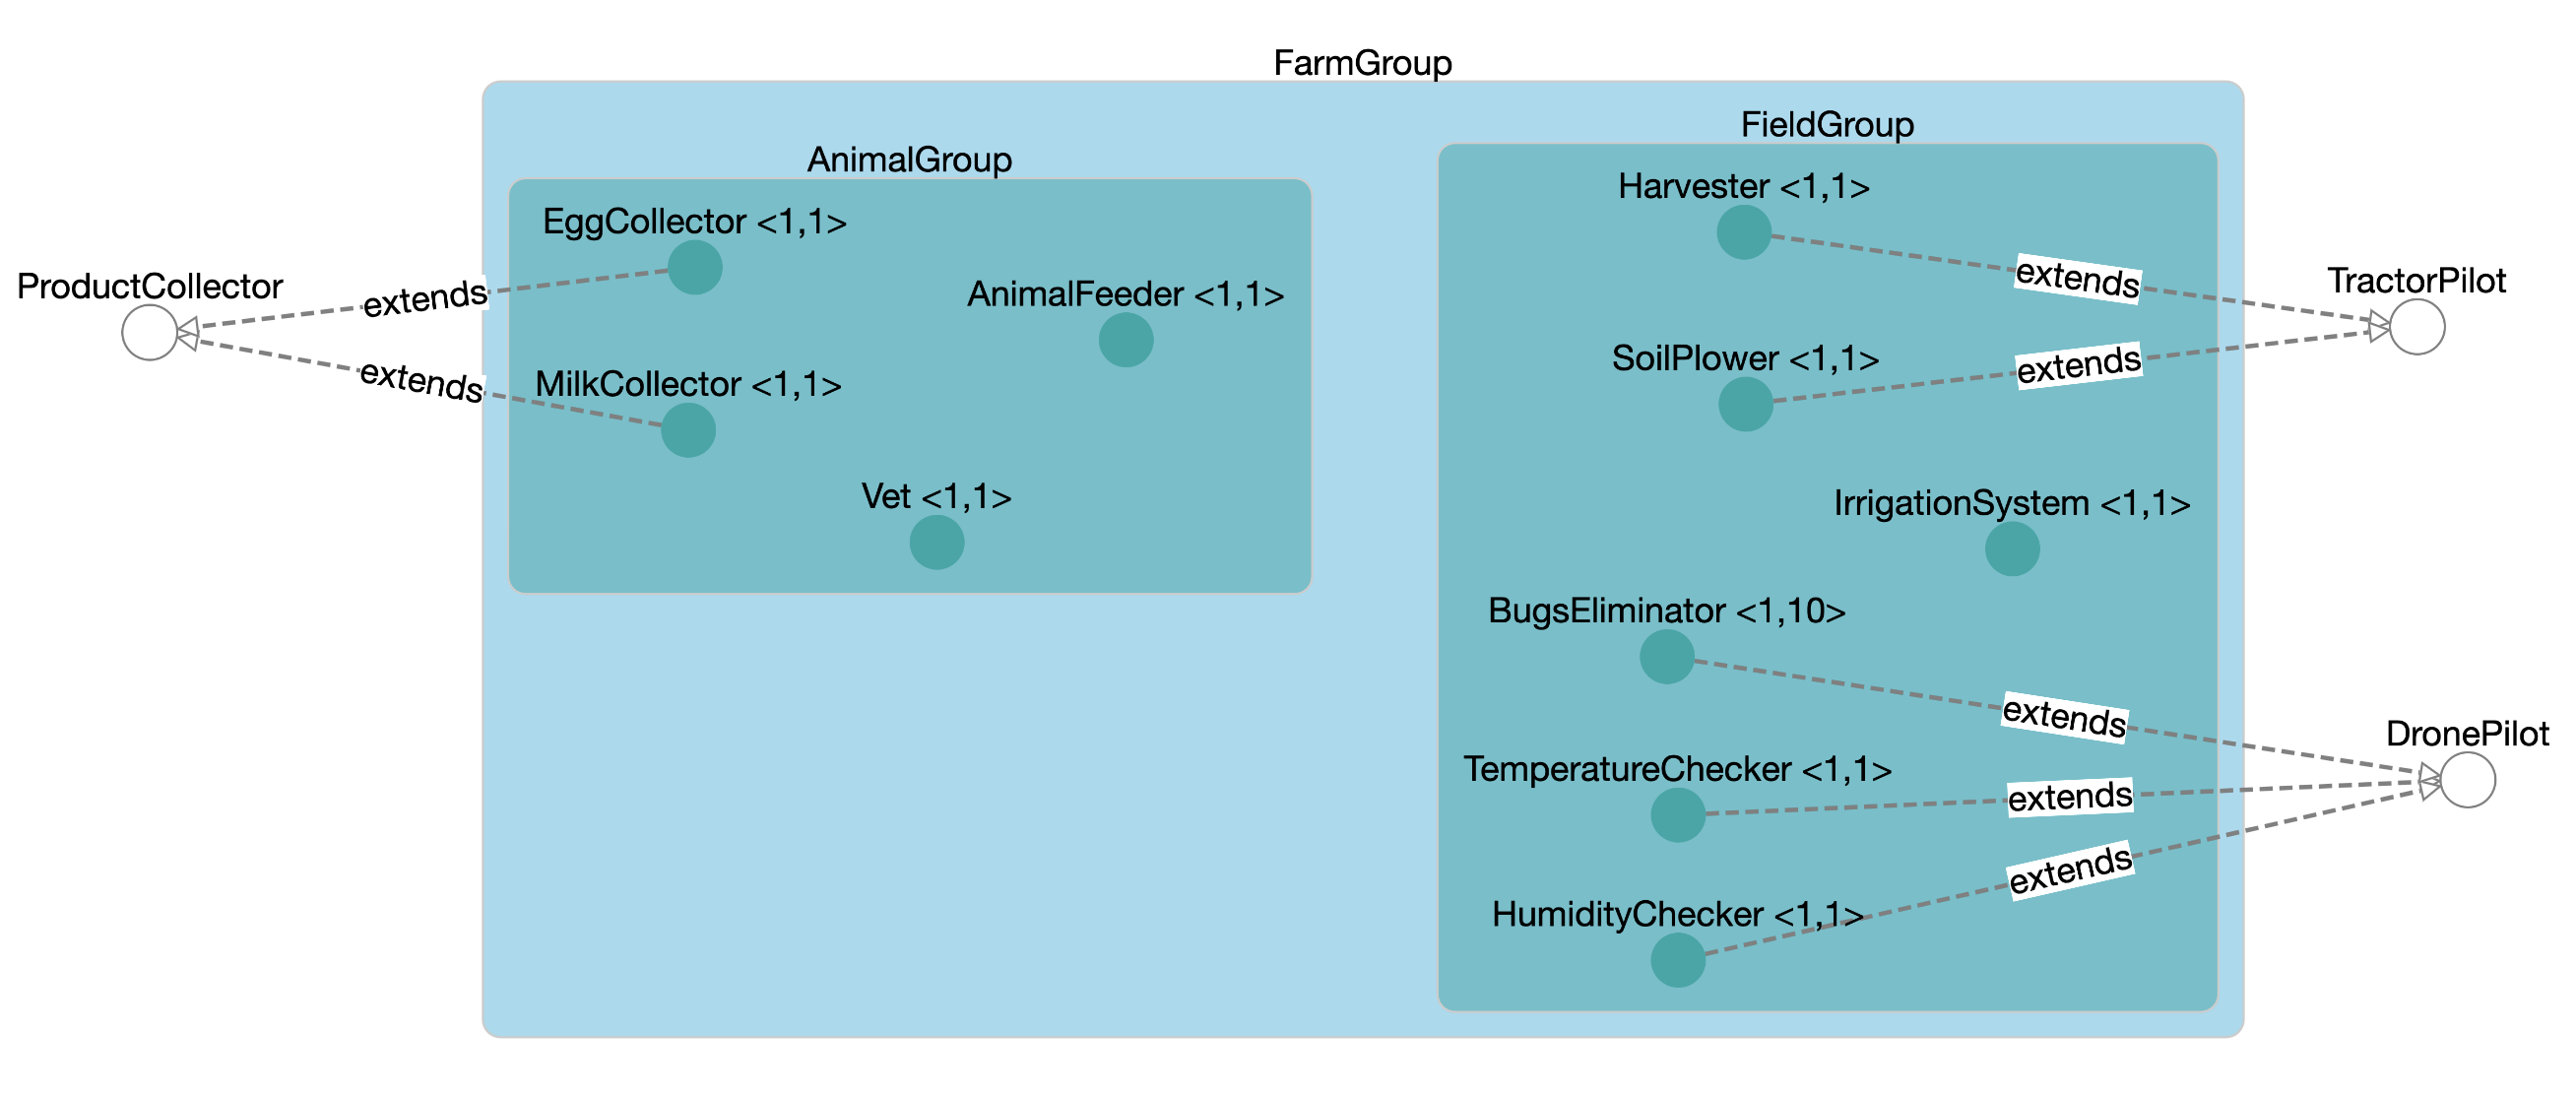
\includegraphics[width=\textwidth]{images/solution-structural.png}
    \caption{Solution for the structure of the organization.}
    \label{fig:solution-structural}
\end{figure}

In \cref{fig:solution-structural} the solution regarding the structure of the organization is presented.
The outermost rectangle represents the \texttt{Farm Group} that contains two subgroups, \texttt{Animal Group} and \texttt{Field Group}, depicted by the two inner rectangles.
The three circles that are not placed inside any group represent the abstract roles \texttt{Product Collector}, \texttt{Tractor Pilot}, and \texttt{Drone Pilot}.
As for the other roles, they are concrete and therefore placed inside their corresponding group.
Some of them extend the abstract roles, as is the case of \texttt{Egg Collector} and \texttt{Milk Collector} that extend \texttt{Product Collector}.
Finally, the cardinality of the roles inside the groups is represented in the form \texttt{\textless min,max\textgreater}.
For instance, the \texttt{Bugs Eliminator} role has to be played by at least 1 agent and at most 10 agents while all the other roles have to be played by exactly 1 agent.

\begin{figure}[H]
    \centering
    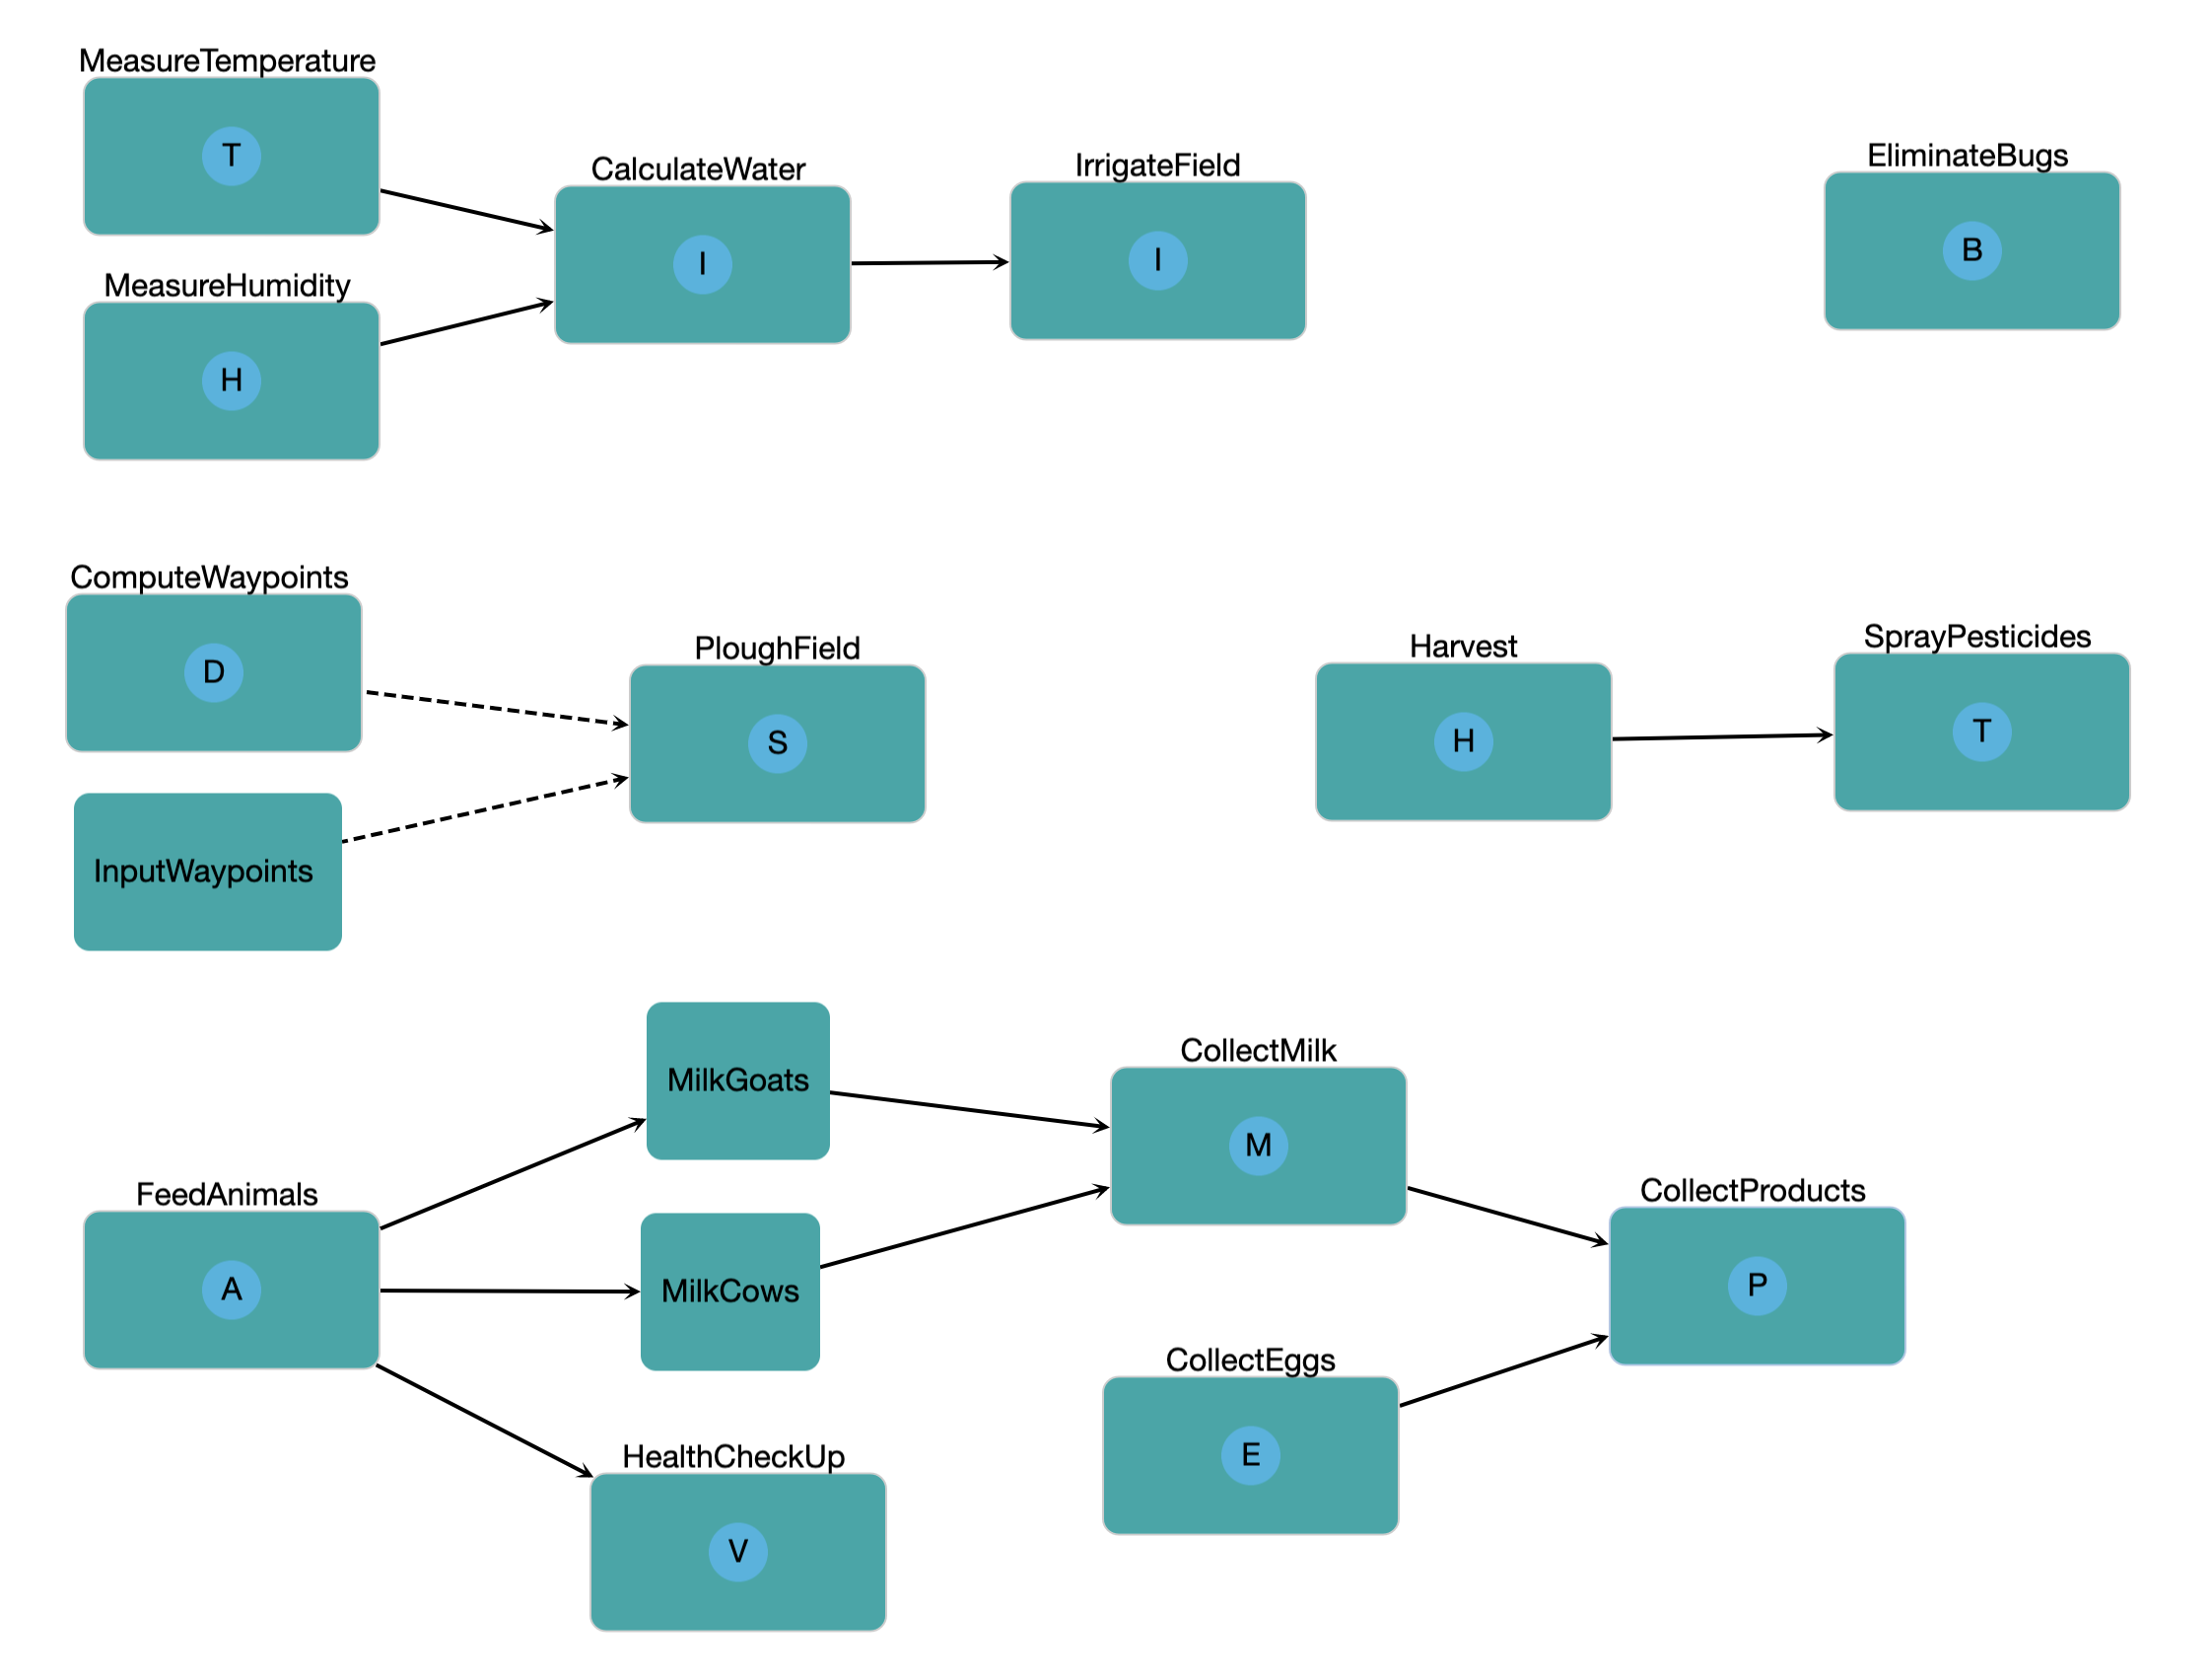
\includegraphics[width=\textwidth]{images/solution-functional.png}
    \caption{Solution for the behavior of the organization.}
    \label{fig:solution-functional}
\end{figure}

As far as the behavior of the organization is concerned, \cref{fig:solution-functional} shows its solution with the visual language.
For instance, the \texttt{Collect Products} goal requires the \texttt{Collect Milk} and \texttt{Collect Eggs} goals to be achieved, therefore, it depends on them with an \textbf{and} relation.
The latter is represented by the solid arrows that connect the enabler goals to the enabled goal.
Indeed, the use of dashed arrows would indicate an \textbf{or} relation, like the one between the \texttt{Compute Waypoints} and \texttt{Input Waypoints} goals and the \texttt{Plough Field} goal.
In turn, the \texttt{Collect Milk} goal requires the \texttt{Milk Cows} and \texttt{Milk Goats} goals to be achieved.
Again, the former depends on the latter goals with an \textbf{and} relation.
Moreover, the \texttt{Milk Cows} and \texttt{Milk Goats} goals need the \texttt{Feed Animals} goals to be achieved in order for them to be pursued.
Finally, the latter goal also enables the \texttt{Health Check-Up} goal.

To conclude, the assignation of the goals to the roles is represented by the presence of the circle corresponding to the role inside the rectangle representing the goal.
For instance, the \texttt{Vet} is responsible for the \texttt{Health Check-Up} goal.

\section{Users' Test}
Due to the shortage of time, it was nearly impossible to gather a large number of users to test the developed visual language.
Moreover, even though the target users for the system are domain experts, finding them and having them test the system would not have been feasible.

Thus, the users' test was performed on a small number of people from the research group.
Since the users have a background in computer science and some of them are familiar with the domain of the scenario, the result was expected to be slightly optimistic but still useful to evaluate the usability of the system.

\subsection{Test Description}
The test consisted in asking the users to provide a solution for the smart-farming scenario using the Web IDE and therefore exploiting the designed visual language.
The vast majority of the users were already familiar with the scenario since they participated in the focus group sessions that helped the design of the visual language itself.
They were also asked to think aloud while they were building the solution, so that possible doubts could be clarified, mainly about the meaning of the concepts of the organization model such as roles, groups, and goals.

After the users had provided their solutions, they were asked to provide feedback through a short questionnaire.
The latter was composed of a few questions about every step of the process, from the identification of the core concepts of the organizations to the use of the Web IDE to build the solution.

The questions were designed to evaluate the usability of the system and the visual language on one hand, and the effectiveness of the organization model on the other, that is the ability of the model to represent the organization in a way that is natural and understandable for the users.
Specifically, the questions were modeled as statements such as \textit{It was easy for me to identify what roles are needed in the organization} and \textit{It was easy for me to create the roles using the IDE}.

The participants were asked to rate the statements on a scale from $1$ to $5$, where $1$ means that they strongly disagreed with the statement and $5$ means that they strongly agreed with the statement.

\subsection{Results}
Even though some of the users needed some hints to get started, all of them were able to provide a solution for the scenario in an acceptable amount of time, with the average time being around $25$ minutes.

All the solutions provided by the users produce a syntactically correct organization specification, which means that no errors will be encountered when the system tries to deploy the organization.
However, the solutions provided by the users are not all necessarily semantically correct, that is, they might not represent the organization in a way that completely matches and satisfies the requirements of the scenario.

What the users most struggled with was the identification of the roles and the groups.
Specifically, they had difficulties in distinguishing the concepts of agents and the roles played by them.
Moreover, some of them had difficulty understanding that roles have to be inserted in groups.
On the other hand, the users easily understood the concept of goals and were able to identify them in the scenario together with the relations between them.

However, once the users were explained the meaning of the concepts and some fundamentals of the organization model, they were able to provide a solution for the scenario in a short amount of time.

As far as the use of the Web IDE is concerned, all the users had no issues in creating the visual components and interacting with them.
What is more, the navigation through the different pages of the IDE was straightforward for all the users.

Therefore, these results show that the visual language is intuitive and that the Web IDE is easy to use.
As far as the organization model is concerned, it appears to be effective in representing the organization powerfully and flexibly, even though some of the users do not inherently reason about organizations in terms of the model's concepts.
Nevertheless, it turned out to be simple enough to be easily understood by the users when they are briefly introduced to the main concepts.

In \cref{fig:questionnaire-results-model} and \cref{fig:questionnaire-results-ui} the ratings of the statements are shown.
The first figure shows the results for the statements related to the organization model, that is the identification of the core concepts of the organization.
On the other hand, the second figure shows the results for the statements related to the use of the Web IDE.
Each color represents a step of the process of the test, that is, the identification and creation of the roles, groups, goals, dependencies among goals, and the assignation of goals to roles, respectively.

According to the feedback provided by the users, the result of the test is extremely positive.
As already stated, the results were expected to be slightly optimistic since the users are familiar with the domain and the organization model.
However, the results show that the organization model is effective in representing the organization and that the visual language is intuitive and easy to use.

Finally, it is worth noting that the user that provided the most complete solution for the scenario was a computer science student who had never heard of MAS organizations before, proving that there is no need for a specific background and previous experience to define one.

\begin{center}
    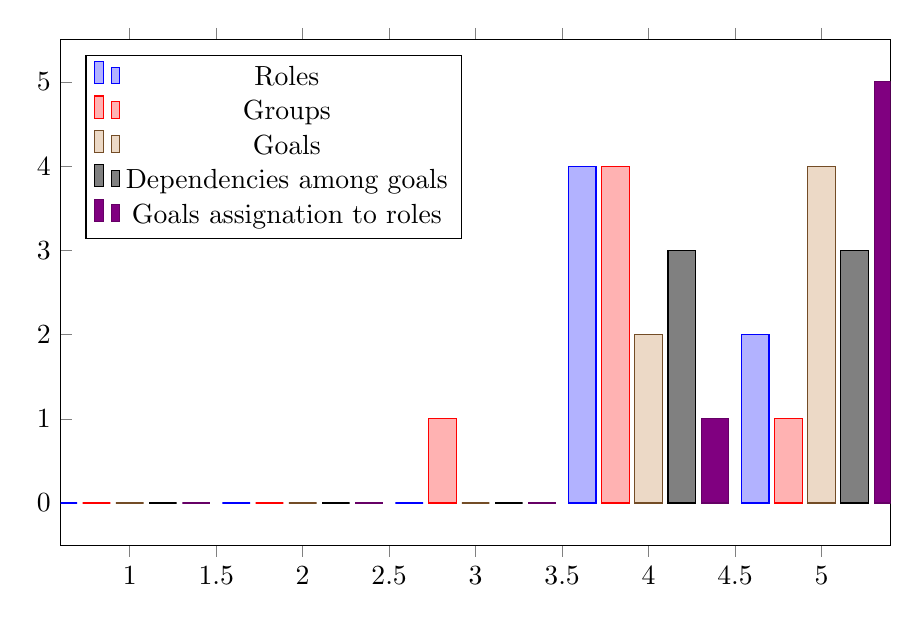
\begin{tikzpicture}
    \begin{axis} [ybar,width=\linewidth,height=8cm,legend pos=north west]
    \addplot coordinates {
        (1,0) 
        (2,0) 
        (3,0) 
        (4,4)
        (5,2)
    };
    \addplot coordinates {
        (1,0) 
        (2,0) 
        (3,1) 
        (4,4)
        (5,1)
    };
    \addplot coordinates {
        (1,0) 
        (2,0) 
        (3,0) 
        (4,2)
        (5,4)
    };
    \addplot coordinates {
        (1,0) 
        (2,0) 
        (3,0) 
        (4,3)
        (5,3)
    };
    \addplot coordinates {
        (1,0) 
        (2,0) 
        (3,0) 
        (4,1)
        (5,5)
    };
    \legend {Roles, Groups, Goals, Dependencies among goals, Goals assignation to roles};
    \end{axis}
    \end{tikzpicture}
    \captionof{figure}{Average rating of the statements concerning the identification of the main concepts of the organization model.}
    \label{fig:questionnaire-results-model}
\end{center}

\begin{center}
    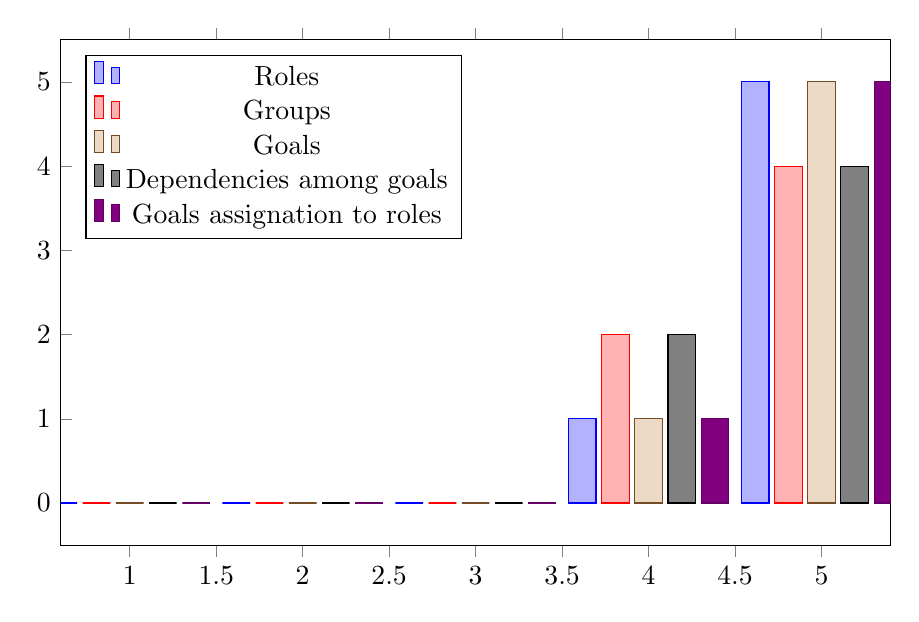
\begin{tikzpicture}
    \begin{axis} [ybar,width=\linewidth,height=8cm,legend pos=north west]
    \addplot coordinates {
        (1,0) 
        (2,0) 
        (3,0) 
        (4,1)
        (5,5)
    };
    \addplot coordinates {
        (1,0) 
        (2,0) 
        (3,0) 
        (4,2)
        (5,4)
    };
    \addplot coordinates {
        (1,0) 
        (2,0) 
        (3,0) 
        (4,1)
        (5,5)
    };
    \addplot coordinates {
        (1,0) 
        (2,0) 
        (3,0) 
        (4,2)
        (5,4)
    };
    \addplot coordinates {
        (1,0) 
        (2,0) 
        (3,0) 
        (4,1)
        (5,5)
    };
    \legend {Roles, Groups, Goals, Dependencies among goals, Goals assignation to roles};
    \end{axis}
    \end{tikzpicture}
    \captionof{figure}{Average rating of the statements concerning the ease of use of the Web IDE when defining the concepts.}
    \label{fig:questionnaire-results-ui}
\end{center}



\chapter*{Conclusions}
\addcontentsline{toc}{chapter}{Conclusions}
\markboth{CONCLUSIONS}{CONCLUSIONS}

\section*{Main Contribution}
As stated multiple times in this document, the main contribution of the thesis work is the application of visual programming techniques to the Multi-Agent Oriented Programming (MAOP) paradigm aiming at overcoming the challenges that come from the coordination of single entities in a way that is accessible by non-technical domain experts.

This project \hl{is} the natural evolution of the previous work from \cite{burattini2022agent} that was also carried out at the University of St.\ Gallen and that was focused on the development of a visual programming paradigm for software agents.
Indeed, it moves a step forward toward the vision for an accessible Integrated Development Environment (IDE) that mixes Multi-Agent Oriented Programming and Hypermedia in a seamless interface for both humans and software agents.

The work culminated in the development of a prototype of the system that was tested and evaluated on a sample of users and gave promising results in terms of usability, user-friendliness, and correctness.
However, a long path was taken to reach this point.

The development steps were first focused on the analysis of the requirements coming from the \textit{IntellIoT} project, the research interest of the hosting group, and the already implemented agent's IDE.
Then the analysis of the tools and technologies used by the research team brought to the identification of \moise{} and the JaCaMo platform as the candidates to implement the solution.

The next step involved the analysis of the \moise{} specifications, its core concepts, and the gathering of a focus group to identify the building blocks of the visual programming language in a way that would be as understandable as possible for the target users.

The implementation of an interface supporting the usage of the visual language followed, alongside the development of a storage and backend to provide the persistence of the organizations created.

Finally, the Web IDE was integrated with the existing runtime environment to allow the execution of the organizations created by the users, therefore allowing the full cycle of development and deployment of the organizations.

The prototype subsequently underwent an evaluation study, first trying to address a rather complex real-world scenario, and then testing the usability of the system with a small sample of users in contact with the tool for the first time and with little to no explanation of its functionalities.

Overall, this thesis brought to the realization of a usable tool that can be used by non-technical users to create and deploy organizations in a way that is accessible and understandable for them.
Most important, this opened a lot of potential directions for future work, as the system is still in its early stages on one hand, and it enables new research threads on the other.

\section*{Open Challenges and Future Work}
Working on a project that touches multiple and diverse research fields, that relies on currently developing technologies, and in an environment that encourages the exploration of new ideas and the interaction with colleagues from different backgrounds and working on different research topics, cannot but result in a continuous flow of new questions and new directions to explore.
Of course, the thesis work cannot follow all the possible paths and therefore a lot can be done to improve the existing solution and expand it.

First of all, the development of the visual language is an ongoing process that requires more iteration than the ones it was possible to carry out to be able to refine the visual building blocks and make them more intuitive and accessible for the users.
Indeed, a lot of work is still needed to find the right visual abstractions to represent the core concepts that might require the exploration of different visual paradigms and the gathering of more feedback from the users.

Moreover, some concepts of the \moise{} specifications were purposefully left out of the visual language, both for time constraints and for the need to keep the language as simple as possible.
However, more advanced users might find it useful to have access to these concepts.
Therefore, a way to extend the visual language to include them should be explored.

As far as the Web IDE is concerned, the current implementation only supports the creation of organizations and their deployment on the runtime environment.
However, it would be extremely interesting to add the possibility to monitor the state and development of the organizations and to provide a way to interact with them.
This way, the user could be involved not only at design time but also at runtime, promoting the human-in-the-loop approach the \textit{IntellIoT} project is based on.

Regarding the runtime environment, for the time being, the user has to manually choose the agents that will participate in the organization and assign them the roles they should play.
However, it would be interesting to explore the possibility of automatically assigning roles to the agents based on their capabilities.
Indeed, some members of the research group are currently working on the development of a framework based on costs and rewards that are assigned to the agents when they adopt a certain role and achieve the goals the role is responsible for.
This is a promising direction toward self-organization and re-organization in Multi-Agent Systems that will be for sure explored in the future.

As far as the technologies used are concerned, lately, a lighter version of \moise{} has been developed, called \moise{} \textit{simple}~\footnote{\url{https://github.com/moise-lang/moise/tree/master/src/main/java/ora4mas/simple}}, that, as the name suggests, should be easier to use for domain experts.
Therefore, it could be fruitful to compare the two approaches and analyze the tradeoffs in terms of user-friendliness and expressiveness.

Hopefully, given the interest in the project from both the research group in St.\ Gallen and the one in Cesena, some of these directions can be explored in future research projects.	
\chapter*{Acknowledgments}
\addcontentsline{toc}{chapter}{Acknowledgments}
\markboth{ACKNOWLEDGMENTS}{ACKNOWLEDGMENTS}

This thesis and my whole student years would not have been the same without the many inspiring people that I have met along the way.
Therefore, I would like to express my gratitude to my mentors, colleagues, and friends that have supported me during this journey.

Firstly, I would like to thank my supervisor, Prof.\ Alessandro Ricci for transmitting to me his passion for his research topics through his enthusiasm when teaching, and for giving me the opportunity to live such a unique experience by putting me in contact with some of the brightest people in the field of Multi-Agent Systems.

Then I would like to thank Samuele Burattini for always being there during the development of this thesis, for your reassurance and support, and for your precious advice.
I wish you all the best for a successful and rewarding academic career.

I would also like to thank everyone I had the pleasure to work with in St.\ Gallen while working on this thesis, especially Prof.\ Simon Mayer, Prof.\ Andrei Ciortea, and J\'{e}r\'{e}my Lem\'{e}e for their continuous support and for introducing and guiding me into the world of research.
From the first day I arrived in St.\ Gallen, you made me feel at home and part of your group, and I am truly grateful for that.
Thank you for all the interesting discussions, the lovely lunch chats, and for sharing your knowledge and experience with me.

Speaking of St.\ Gallen, I would also like to thank my flatmate Sebastian and my friends Lukas and Jennifer for making my stay there so enjoyable, letting me have some fun after long days of work, and supporting me when work was overwhelming and through sad and difficult times.
In such a short time, we have been able to share so much and you have become such an important part of my life.

I would wish to thank my family for their unconditional everyday support, the help they always provide me with, and for allowing me to keep studying and following my passions and dreams.
I know that sometimes I am not the most open and outgoing person, but I truly appreciate all the love and care you give me.

Even though probably words are not enough to express my gratitude, I still want to try and thank the members of what I call my second family.
First of all, Simone whom I met during my first year of university and who had the burden to put up with me since.
Hopefully, we can yell at each other some more when working together on other projects in the future.
Equally, I would like to thank Marta and Martina.
We have shared quite possibly all the joy and sorrow of our master's degree.
Thank you for always being by my side and I hope I was only half as good a friend to you as you have been to me.

Last but not least, I would like to thank my colleagues and friends that have been with me during my student years and that have made my time at university so special.



	
\backmatter	

\bibliography{bibliography}{}
\bibliographystyle{plain}

\end{document}